\chapter{Mitigation Strategies}
\label{chap:mitigationstrats}

In this Chapter 'Mitigation Strategies' solutions to the discovered problems are described. In the first instance, one will illustrate the structural solutions for bank erosion. Moving on to different strategies, the choice was made to investigate how Nature-based solutions could be implemented. On the one hand, the principle of Nature-based solution was applied to mitigating the impact of dry sand mining. On the other hand, it was applied to mitigate the impact of river sand mining, thus looking at bank erosion once again. 

\section{Structural Solutions for Bank Erosion}
\label{section_8.2}

Several retaining structures that can be used to stabilize the river banks. Possibilities include:
\begin{itemize}
    \item Sheet pile wall\\
    Sheet pile walls are a common retaining structure and consist of vertical barriers made of interlocking sections. They are a lightweight option and can be removed, which makes them reusable across multiple projects. Another advantage is the fact that installation is relatively easy and therefore cheap. However, sheet pile walls also have limitations. In hard soils and soils with boulders or cobbles, installation becomes difficult. Further, installation can disturb nearby areas through sounds and vibrations. These vibrations can even cause settlements to occur \autocite{korffReaderDeepExcavations2023}.

    \item Diaphragm wall\\
    Diaphragm walls are deep, reinforced concrete retaining structures. They provide excellent structural stability and are capable of resisting significant lateral soil and water pressures. One of their key advantages is water tightness, as they effectively prevent groundwater seepage. They are also suitable for a wide range of soil conditions, and offer durability due to the use of reinforced concrete. On the downside, they are costly to build and require significant time and space due to the specialized equipment, skilled labor, and extensive excavation work that is needed \autocite{korffReaderDeepExcavations2023}.
    
    \item Precast concrete wall\\
    Precast concrete walls are constructed by manufacturing structural elements in a factory environment before transporting them to the construction site. This process allows for superior quality control. Moreover, precast construction can significantly speed up project timelines, as elements are produced in large quantities and quickly installed on-site. Precast concrete offers a long service life with minimal maintenance. Drawbacks of precast concrete walls include: the elements are heavy and thus require specialized transportation and installation equipment \autocite{mcneilengineeringAdvantagesDisadvantagesUsing2023}. Further, the production and transport processes have notable environmental impacts, and repairs or replacements can be complex and costly.

    \item Auger pile wall or soldier pile wall\\
    Auger pile walls and soldier pile walls are widely used in construction for retaining slopes. Auger pile walls are formed by drilling and casting concrete in place, while soldier pile walls consist of vertical steel or timber H-piles with horizontal boards or panels placed between them. They are generally cost-effective solutions that generate minimal vibrations, making them suitable for urban areas and sites sensitive to noise or disturbance. Both systems offer flexibility, allowing adjustments to pile placement, size, and depth to suit specific project requirements. However, leakage between adjacent piles is a relevant risk when it comes to these types of walls \autocite{korffReaderDeepExcavations2023}. Maintaining proper overlap between piles is also critical to ensure structural stability and continuity of the wall.
\end{itemize}

In Table \ref{tab:compstruct}, the different structural solutions are summarized and are scored on different relevant criteria.

\begin{table}[H]
\centering
\caption{Comparison of structural solutions}
\resizebox{\textwidth}{!}{%
\begin{tabular}{lcccccccc}
\hline
Method & Installation & Price & Resistance & Versatility & Disturbance & Water tightness & Durability & Sustainability \\
\hline
Sheet pile wall & ++ & + & + & - & - & 0 & + & ++ \\
Diaphragm wall  & -- & -- & ++ & ++ & + & ++ & ++ & - \\
Precast concrete wall & - & - & ++ & 0 & ++ & + & + & -- \\
Auger/Soldier pile wall & + & ++ & 0 & + & ++ & -- & - & 0 \\
\hline
\end{tabular}%
}
\label{tab:compstruct}
\end{table}

As can be seen in Table \ref{tab:compstruct}, pile walls score low on water tightness and durability. The area of interest is located in a delta and hence high groundwater levels are to be expected. Therefore, water tightness must be guaranteed. Since the pile walls don't offer this certainty, this option is not further discussed. The diaphragm wall, on the other hand, offers great water tightness but installation is a far bigger challenge for this method. The benefits that the diaphragm wall offers, great resistance and low disturbance being the most relevant ones, do not outweigh the cons: the large amounts of time, space and budget needed to construct them. The same is true for the precast concrete wall: the heavy elements ask for a specialized and expensive installation procedure. The specialized equipment and experience is possibly not available or expensive, which means the precast concrete walls are not a viable option.

As a structural solution, the sheet pile walls are chosen. These elements score high on ease of installation and sustainability (parts can be removed and reused) and price, resistance and durability are also pros of this method. Disturbance is one of the main concerns related to sheet pile walls, but since the area of interest is in a scarcely populated area, this is not necessarily problematic. Another concern is the low versatility: installation is only possible if soils are not too hard. However, since installation will be executed in a delta with relatively soft soil (see xx), this should not be a major concern for this project.

\section{Sheet Pile}
\label{section:sheet_pile_wall}

Sheet pile walls are frequently used for excavations, waterfront structures, highway structures, flood protection schemes, and bridge abutments. Steel sheet pile walls are mainly used because they offer a wide variety of combinations and profiles. These profiles achieve high moments of resistance while still meeting the structural design requirements. Their engineering advantages include their suitability for water use, a favorable ratio of steel cross-section to moment of resistance, and rapid site progress. These factors make them both functional and economical, which supports their widespread use (Handbook).

\subsubsection{Cantilever and anchored}

The types of steel sheet pile walls most used in practice are cantilever and anchored sheet piles. Cantilever sheet piles are used as flood or earth retaining walls with heights ranging between 3 and 5 meters. They get their support from the ground and foundation soils, which can be seen in Figure \ref{fig:sheetpiles}. The anchored sheet piles can be used when the heights of cantilever sheet piles are exceeded or when the design is based on lateral deflections. However, for anchored sheet piles, a free horizontal distance should be incorporated for the installation of the anchor, shown in Figure \ref{fig:sheetpiles} (EM-1110).

\begin{figure}[H]
    \centering
    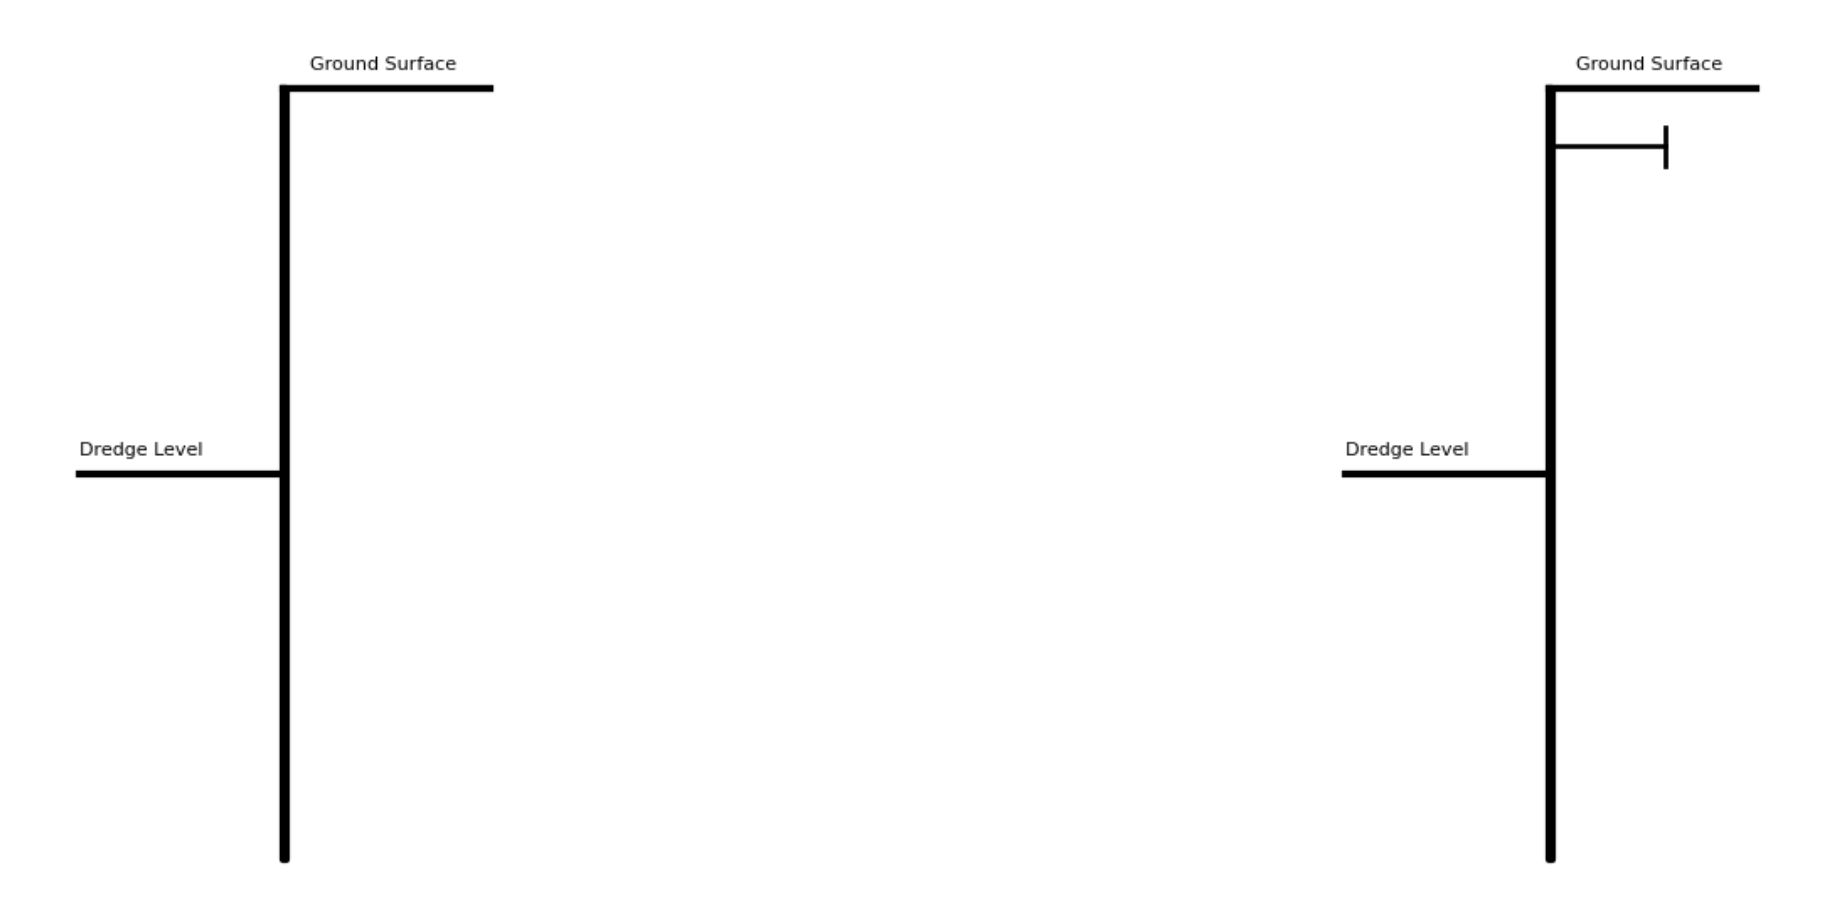
\includegraphics[width=0.70\linewidth]{figures/ch8/cantilever_anchored.png}
    \caption{Cantilever and anchored sheet pile wall}
    \label{fig:sheetpiles}
\end{figure}

% DEZE FIGUUR WELLICHT ZELF MAKEN IN PYTHON. CANTILEVER HEB IK AL. ANCHORED NOG EVEN MAKEN SIMPEL.

\subsubsection{Materials}

Sheet pile walls can be made of multiple materials, like steel, concrete, or wood. For the design in this report, steel will be used as the advantages outweigh the disadvantages and are more suitable than concrete or wood. Concrete will have a longer service life, however, it will have higher initial costs compared to steel, and the installation of concrete walls is more difficult. Wooden walls can be used for shorter heights and temporary structures.  As discussed in Section \ref{section_8.2}, the advantages of steel sheet piles make it the most common material because of the strength, light weight, and long service life, in combination with the favorable ratio of cross-section and moment of resistance (EM-1110). The following section will outline the key steel properties relevant to the design.

\subsubsection{Sections and interlocks}

The sections and interlocks for the steel sheet pile walls are crucial for completing a wall when  using it for waterfront structures. Figure \ref{fig:sections_sheetpiles} shows typical steel sections widely used and goes by the names of U and Z sections. In this figure, the interlocks, which give the sections their strength, can also be seen. The interlocks of the U sections are on the neutral axis, and the ones for the Z sections are not. In the neutral axis, the maximum shear stress is obtained, which means the interlocks should be welded or crimped to obtain the full moment of resistance. When sections meet with water, the walls must be watertight. This can be done with plastic compound materials filling the interlocks or using a preformed polyurethane interlock seal. 

% NOG EEN BETERE FOTO LATEN ZIEN VAN INTERLOCKS

\begin{figure}[H]
    \centering
    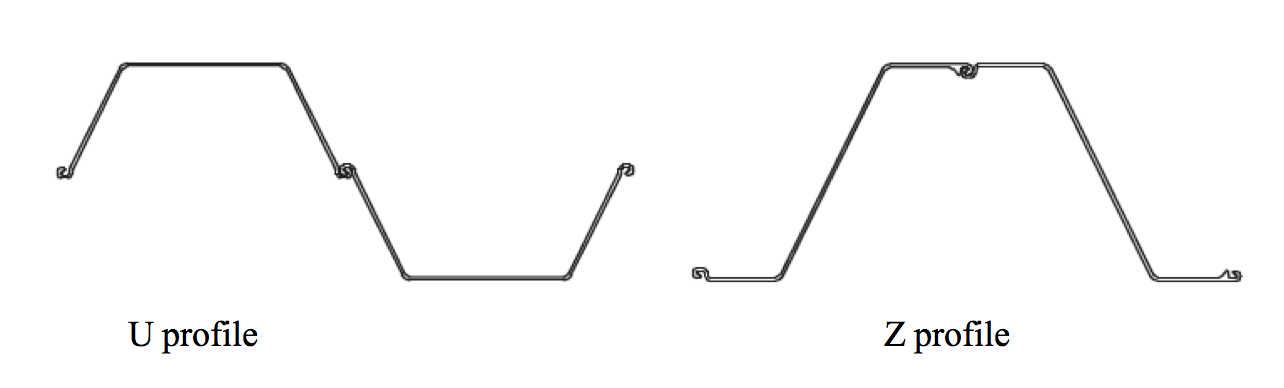
\includegraphics[width=0.50\linewidth]{figures/ch8/u_profile_z_profile.png}
    \caption{U and Z sections}
    \label{fig:sections_sheetpiles}
\end{figure}

\subsubsection{Steel properties}

Steel will be the material used for the sheet piles. The properties of steel, as a homogeneous material, will be briefly introduced. Steel is an elastic material with a favorable strength-to-weight ratio and a tensile strength ranging between 300 $N/mm^{2}$ and 2000 $N/mm^{2}$. Next, the stress-strain behavior and specific mechanical properties of steel will be discussed.  

The stress-strain behavior of steel can be seen in Figure \ref{fig:stress_strain_steel}. The range of elasticity depends on the grade of steel, and the elastic modulus for steel, $E$, is 210000 $N/mm^{2}$. In Figure \ref{fig:stress_strain_steel}, $f_{y}$ is the yield strength, which is the value where the stress will be constant, drop, or reach a strain of 0.2\% when the load is removed. Furthermore, $f_{u}$ is the tensile strength, which is according to the grade of steel (Handbook). The mechanical properties of the steel used for the sheet piles are shown in Table \ref{tab:steel_materialproperties}.

% MOOI EN DUIDELIJK STUK SCHRIJVEN OVER DE STRESS-STRAIN RELATIE WAARIN DUIDELIJK WORDT WAT VOOR EEN MATERIAAL STAAL IS EN HOE HET ZICH GEDRAAGD. OOK BACK-UP VAN PAPERS ERIN VERWERKEN.

\begin{figure}[H]
    \centering
    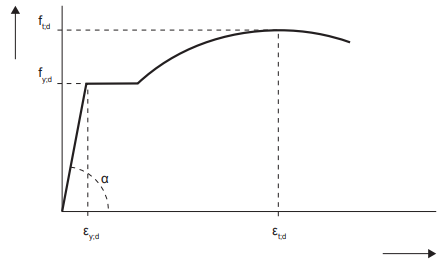
\includegraphics[width=0.50\linewidth]{figures/ch8/stress_strain_steel.png}
    \caption{Stress-strain relation steel}
    \label{fig:stress_strain_steel}
\end{figure}

\begin{table}[H]
  \centering
  \caption{Mechanical properties by steel grade}
  \label{tab:steel_materialproperties}
  \small
  \renewcommand{\arraystretch}{1.15}
  \begin{tabularx}{\linewidth}{@{}l l l l@{}}
    \toprule
    Steel grade &
    \makecell{Tensile strength $f_{u}\,[\mathrm{N/mm}^{2}]$} &
    \makecell{Yield strength $f_{y}\,[\mathrm{N/mm}^{2}]$} &
    \makecell{Elongation at failure $\varepsilon_{u}\,[\%]$} \\
    \midrule
    S 240 GP & 340 & 240 & 26 \\
    S 270 GP & 410 & 270 & 24 \\
    S 320 GP & 440 & 320 & 23 \\
    S 355 GP & 480 & 355 & 22 \\
    S 390 GP & 490 & 390 & 20 \\
    S 430 GP & 510 & 430 & 19 \\
    \bottomrule
  \end{tabularx}
\end{table}

\textit{Hot-rolled steel}

Steel sheet piles are made of hot-rolled sections, which are made in the process of heating steel to temperatures of 900 $^{\circ}$C  above the recrystallization temperature before rolling. This allows for the various shapes and larger sizes that are of importance with sheet piles (Chesterfield). Compared with cold-rolled sections, hot-rolled sections have a slightly rougher surface and are cheaper because reheating is not required (Chesterfield). 

% EVEN HOT ROLLED BESPREKEN. WAT, WAAROM, HOEZO?

\textit{Sustainability}

In Table \ref{tab:env_impacts}, an overview of the materials, concrete, steel and timber is provided in relation to the emissions $CO_{2}$ and the energy consumption. As can be seen from the table, the production and use of steel is the least sustainable. However, the choice of steel is made based on the advantages of the profile and its fast installation. In this paragraph, research is conducted to assess which profile is most sustainable for the design of the steel sheet piles.

\begin{table}[H]
  \centering
  \caption{Environmental impacts by material}
  \label{tab:env_impacts}
  \small
  \setlength{\tabcolsep}{6pt}
  \renewcommand{\arraystretch}{1.15}
  \begin{tabularx}{\linewidth}{@{}l l l@{}}
    \toprule
    Material &
    CO$_2$ emissions (kg CO$_2$e per ton) &
    Energy consumption (MJ per ton) \\
    \midrule
    Concrete & 100 to 200 & 1200 to 1600 \\
    Steel    & 1800 to 2000 & 20000 to 35000 \\
    Timber   & -600 to -1200 & 500 to 1000 \\
    \bottomrule
  \end{tabularx}
\end{table}

A sustainable solution for sheet piles is found in the EPD ‘EcoSheetPiles™ Plus’ from ArcelorMittal. This steel sheet pile is produced by an electric arc furnace. In this process, 100\% renewable electricity and 100\% scrap steel are used for production (ArcelorMittal). Compared to the blast furnace, the production of $CO_{2}$ gasses is significantly reduced, as can be seen in Figure \ref{fig:eaf_bof}.

\begin{figure}[H]
    \centering
    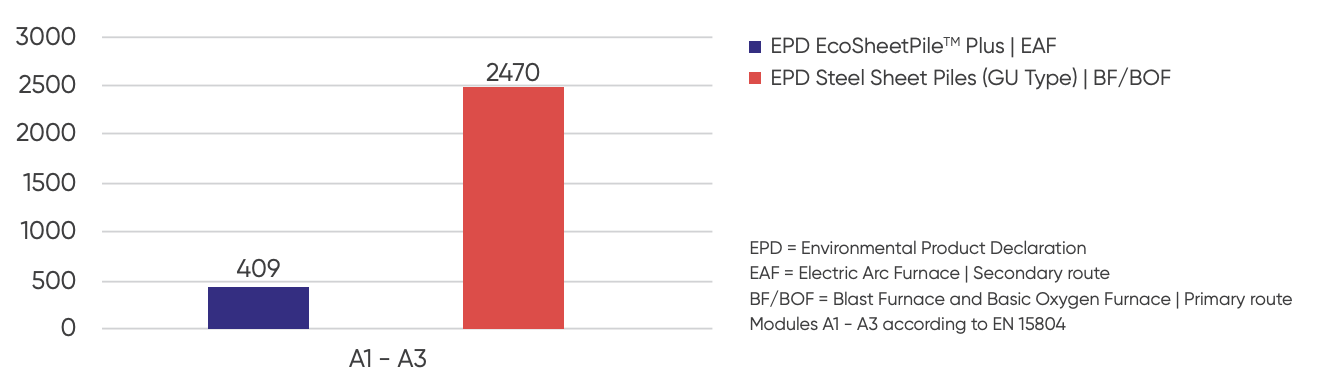
\includegraphics[width=0.70\linewidth]{figures/ch8/eaf_bof.png}
    \caption{Global warming potential [kg CO2e/t sheet pil] (ArcelorMittal)}
    \label{fig:eaf_bof}
\end{figure}

% NOG EVEN GOED UITZOEKEN NAAR WELKE MATERIAL PROPERTIES BELANGRIJK KUNNEN ZIJN. OOK EVEN SUSTAINABILITY IN ACHT NEMEN MET DE GEVONDEN DOCUMENTEN. WELLICHT EEN KOPJE SUSTAINABILITY EN WAT PLOTJES LATEN ZIEN.

\subsubsection{Failure mechanisms}

\begin{figure}[H]
    \centering
    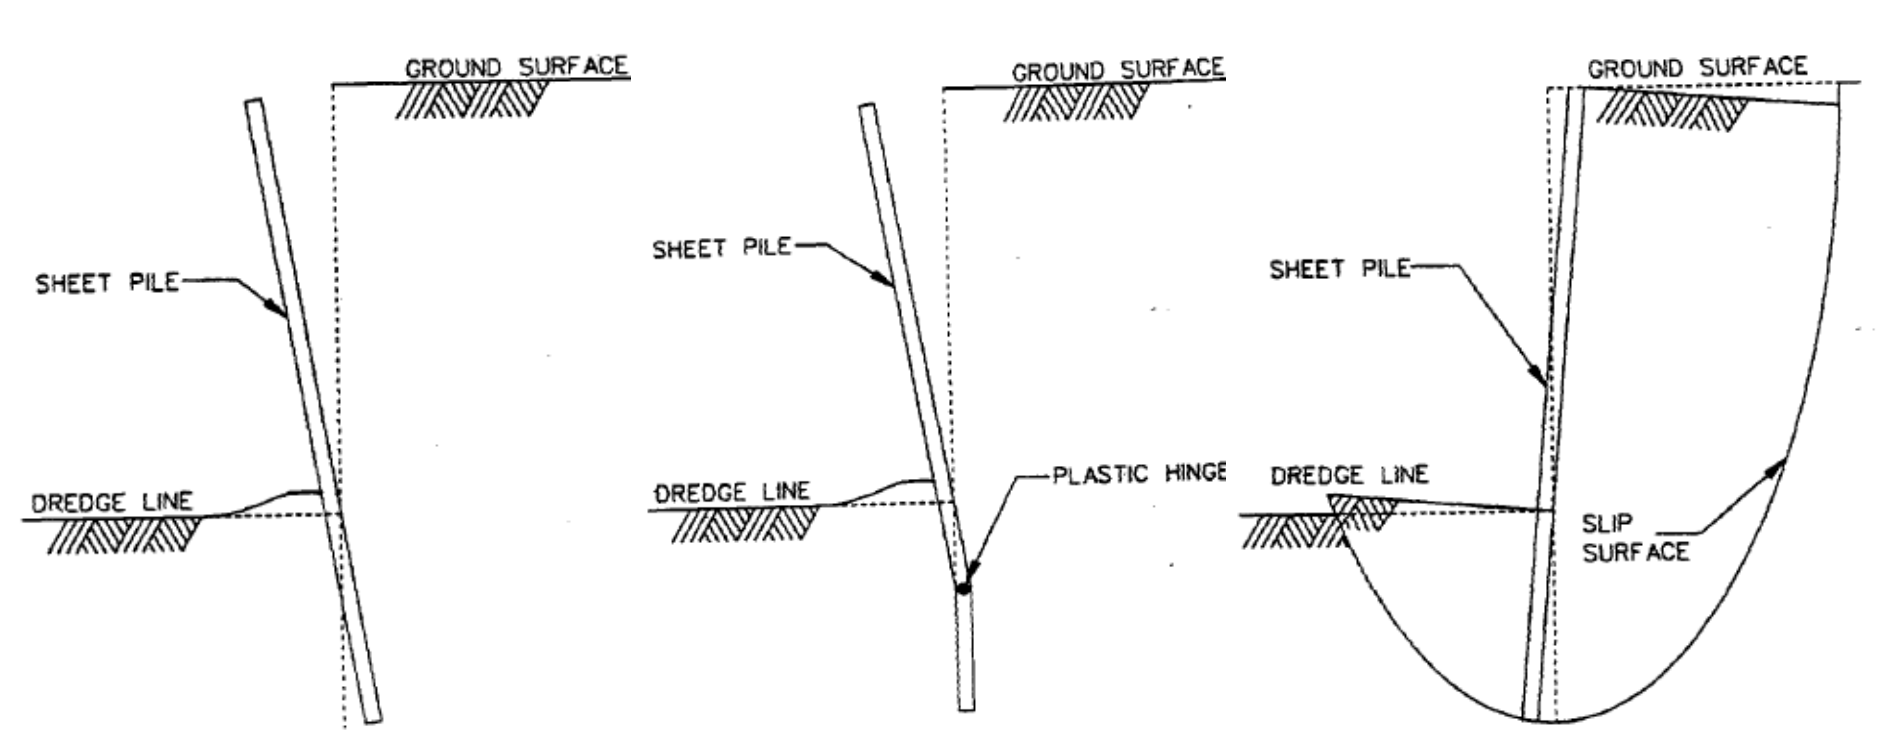
\includegraphics[width=0.70\linewidth]{figures/ch8/failure_mechanisms.png}
    \caption{Failure mechanisms cantilever sheet pile wall}
    \label{fig:failure_mechanisms_sheetpiles}
\end{figure}

% HIER NOG DE FAILURE MECHANISMS BESPREKEN. EVEN KIJKEN WAAROM IK HIER AL ALLEEN DE CANTILEVER LAAT ZIEN. WELLICHT OOK DIE VAN DE ANCHORED LATEN ZIEN OMDAT DE KEUZE PAS VERDER WORDT GEMAAKT.

\newpage

\subsection{Geotechnical parameters}

For the design, the soil layers, including their geotechnical parameters, should be known. In Paragraph \ref{par:geology}, the geological background for the area of interest is explained, and this serves as the basis for deriving the soil layers and parameters. The borehole in Figure \ref{fig:borehole} is deemed the most relevant source. The borehole shows a top layer with fine/medium sands. Below, clay/clayey sand can be found, and the bottom layer consists of medium sand. This is in accordance with the geological profile that was provided before in Figure \ref{fig:geolprofile}, which describes a transition from near-surface beach ridges, dunes, beach plains, and delta sub-aerial facies to deeper open estuaries and marine deposists. The top deposits help declare the presence of sandy deposits at the top of the borehole and the layers of clay/clayey sand below correspond to estuarine deposits. Finally, old marine/fluvial deposits were likely compacted and lead to the layer of medium sand found at the bottom of the borehole.

Because of the resemblance between the local borehole and the geological profile given before, the layering as shown in Figure \ref{fig:borehole} is deemed representative for the whole study area. Based on this layering the relevant parameters can be derived, the result is shown in Table \ref{tab:soil_layers}.

\begin{table}[H]
  \centering
  \caption{Characteristic values soil}
  \label{tab:soil_layers}
  \small
  \setlength{\tabcolsep}{6pt}
  \renewcommand{\arraystretch}{1.15}
  \begin{tabularx}{\linewidth}{@{}p{1.6cm}l p{1.6cm}*{5}{Y}@{}}
    \toprule
    Layer &
    Soil type &
    Depth [m] &
    $\gamma_d\,[\mathrm{kN/m}^3]$ &
    $\gamma_{\!sat}\,[\mathrm{kN/m}^3]$ &
    $\varphi'\,[{}^\circ]$ &
    ${c'}\,[\mathrm{kPa}]$ &
    ${c_u}\,[\mathrm{kPa}]$ \\
    \midrule
    1 & Fill               & 0.0 - 2.0   & 12 & 12 & 15.0 & 2.5 & 20 \\
    2 & Fine/medium sand   & 2.0 - 7.0   & 17 & 19 & 30.0 & 0.0 & \textemdash \\
    3 & Clay               & 7.0 - 10.0  & 14 & 14 & 17.5 & 0.0 & 25 \\
    4 & Clayey sand        & 10.0 - 15.0 & 18 & 20 & 25.0 & 0.0 & \textemdash \\
    5 & Clay               & 15.0 - 16.0 & 14 & 14 & 17.5 & 0.0 & 25 \\
    6 & Clayey sand        & 16.0 - 17.5 & 18 & 20 & 25.0 & 0.0 & \textemdash \\
    7 & Medium sand        & 17.5 - 32.0 & 18 & 20 & 32.5 & 0.0 & \textemdash \\
    \bottomrule
  \end{tabularx}
\end{table}

% TABEL VERBETEREN NAAR DE JUISTE FORMAT. EVEN KIJKEN NAAR DE TABEL UIT PYTHON

% \begin{table}[H]
%   \centering
%   \caption{Design values soil DA1-2}
%   \label{tab:soil_layers}
%   \small
%   \setlength{\tabcolsep}{6pt}
%   \renewcommand{\arraystretch}{1.15}
%   \begin{tabularx}{\linewidth}{@{}p{1.6cm}l p{1.6cm}*{5}{Y}@{}}
%     \toprule
%     Layer &
%     Soil type &
%     Depth [m] &
%     $\gamma_d\,[\mathrm{kN/m}^3]$ &
%     $\gamma_{\!sat}\,[\mathrm{kN/m}^3]$ &
%     $\varphi'\,[{}^\circ]$ &
%     ${c'}\,[\mathrm{kPa}]$ &
%     ${c_u}\,[\mathrm{kPa}]$ \\
%     \midrule
%     1 & Fill               & 0.0 - 2.0   & 12 & 12 & 12.1 & 2.5 & 20 \\
%     2 & Fine/medium sand   & 2.0 - 7.0   & 17 & 19 & 24.8 & 0.0 & \textemdash \\
%     3 & Clay               & 7.0 - 10.0  & 14 & 14 & 14.2 & 0.0 & 17.9 \\
%     4 & Clayey sand        & 10.0 - 15.0 & 18 & 20 & 20.5 & 0.0 & \textemdash \\
%     5 & Clay               & 15.0 - 16.0 & 14 & 14 & 14.2 & 0.0 & 17.9 \\
%     6 & Clayey sand        & 16.0 - 17.5 & 18 & 20 & 20.5 & 0.0 & \textemdash \\
%     7 & Medium sand        & 17.5 - 32.0 & 18 & 20 & 27.0 & 0.0 & \textemdash \\
%     \bottomrule
%   \end{tabularx}
% \end{table}


The parameters in Table \ref{tab:soil_layers} were derived from the Eurocode \autocite{stichtingkoninklijknederlandsnormalisatieinstituutNederlandseNormNEN2025}. Because of limited knowledge on soil characteristics, conservative estimates were made based on this code. In the borehole, no explicit information is given on the top fill layer. Therefore, conservative parameters were assumed based on typical values for organic topsoil. As derived from the borehole and the overview in Table \ref{tab:soil_layers}, the soil profile with the specific layers and properties is shown in Figure \ref{fig:soil_profile_cross_section}. 

\begin{figure}[H]
    \centering
    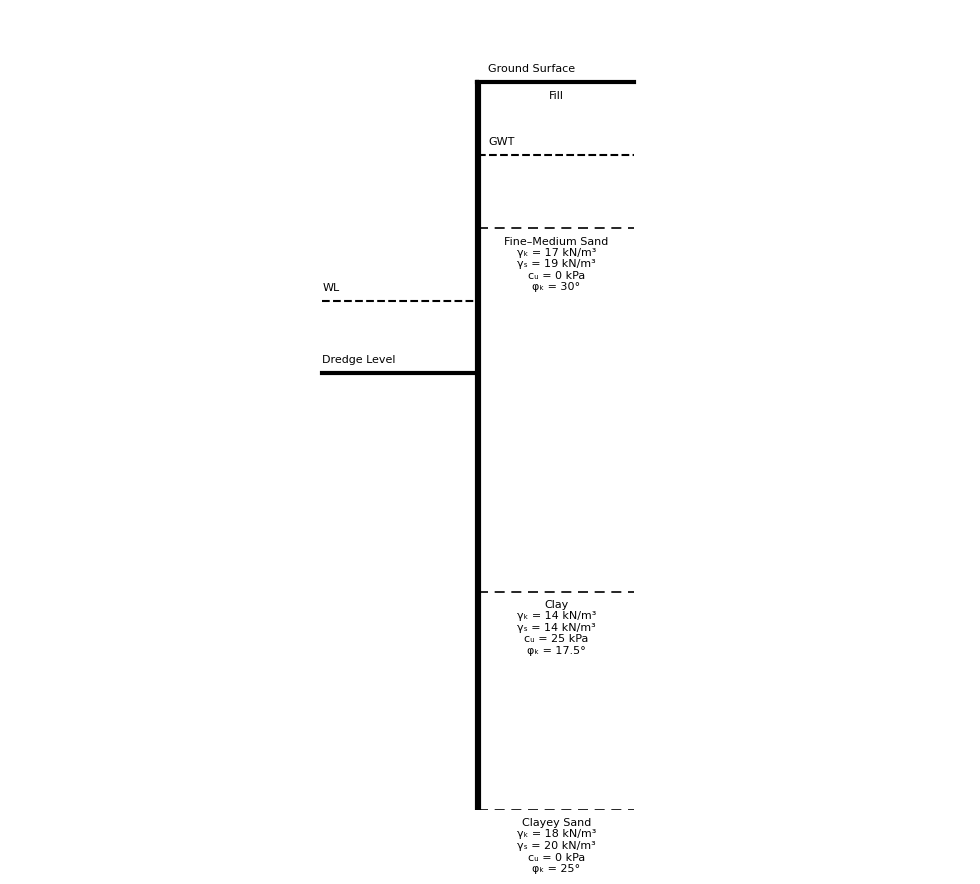
\includegraphics[width=0.55\linewidth]{figures/ch8/soil_profile.png}
    \caption{Soil profile and propeties}
    \label{fig:soil_profile_cross_section}
\end{figure}

\subsection{Hydraulic parameters}
\label{section:hydraulic_parameters}

In addition to the geotechnical values and parameters, the design of the cantilever sheet pile wall is also based on the hydraulic parameters and values. In this design, the sheet pile wall is located in open water and has a groundwater table. Because of this, the hydrostatic pressure will be acting on both sides of the wall. The water level of the river and the groundwater may differ in level, and when this is the case, an excess of hydrostatic pressure will be acting on the sheet pile. 

Apart from this, the height of the river is of importance. This value was determined from the bathymetry of the river at the critical location. In Figure XX, the bathymetry is provided, and the corresponding value is visible. For the design of the sheet pile, "the most unfavorable that could occur during the design working life of the structure" has to be considered. In this report, the fluctuations of the water levels are set at $2.0 \ m$. 


% AANNAMES

% RIVERBED OP 1.5M DOOR DE AFSTAND TUSSEN OEVER EN BATH. WATER LEVEL, GEINTERPOLEERDE METINGEN TUSSEN BRAZO LARGO EN IBICUY VAN ELEVATIONS. WATERLEVEL IS UITGEDRUKT IN ELEVATION EN DAT IS METER ING. DESIGN WATER LEVEL IS GEBASEERD OP 95% LOWER BOUND VAN DE CONFIDENCE INTERVAL. NEEM AAN OP BASIS VAN FOTO DAT HET HOOGTE VERSCHIL MINIMAAL EEN 1.0-1.5M, DUS DAAROM EEN DESIGN WAARDE VAN 2.5M IGN MAAIVELD. 

% KWA FIGUREN: BATHEMTRY PLUS CROSS-SECTION LOCATION. INFORMATIE OVER DE GEBRUIKTE BT STAAT IN SECTION 7.1.1. 

% TIMESERIES VAN WATER ELEVATIONS. HIERVAN ZEGGEN DAT HET HISTORISCHE DATA IS MET 20MIN INTERVAL VOOR DATA PUNTEN. OVER 4 JAAR.

% HIER NOG EEN BATHERMTRY TOEVOEGEN OF VERWIJZEN NAAR HYDRAULIC SECTION. EVEN KIJKEN WAT TE DOEN MET HIER AL AANGEVEN DAT WE 2 METER WATER DALING KUNNEN HEBBEN EN DIT DE MEEST ONGUNSTIGE SITUATIE IS.

% \begin{figure}[H]
%     \centering
%     \begin{subfigure}[b]{0.45\textwidth}
%         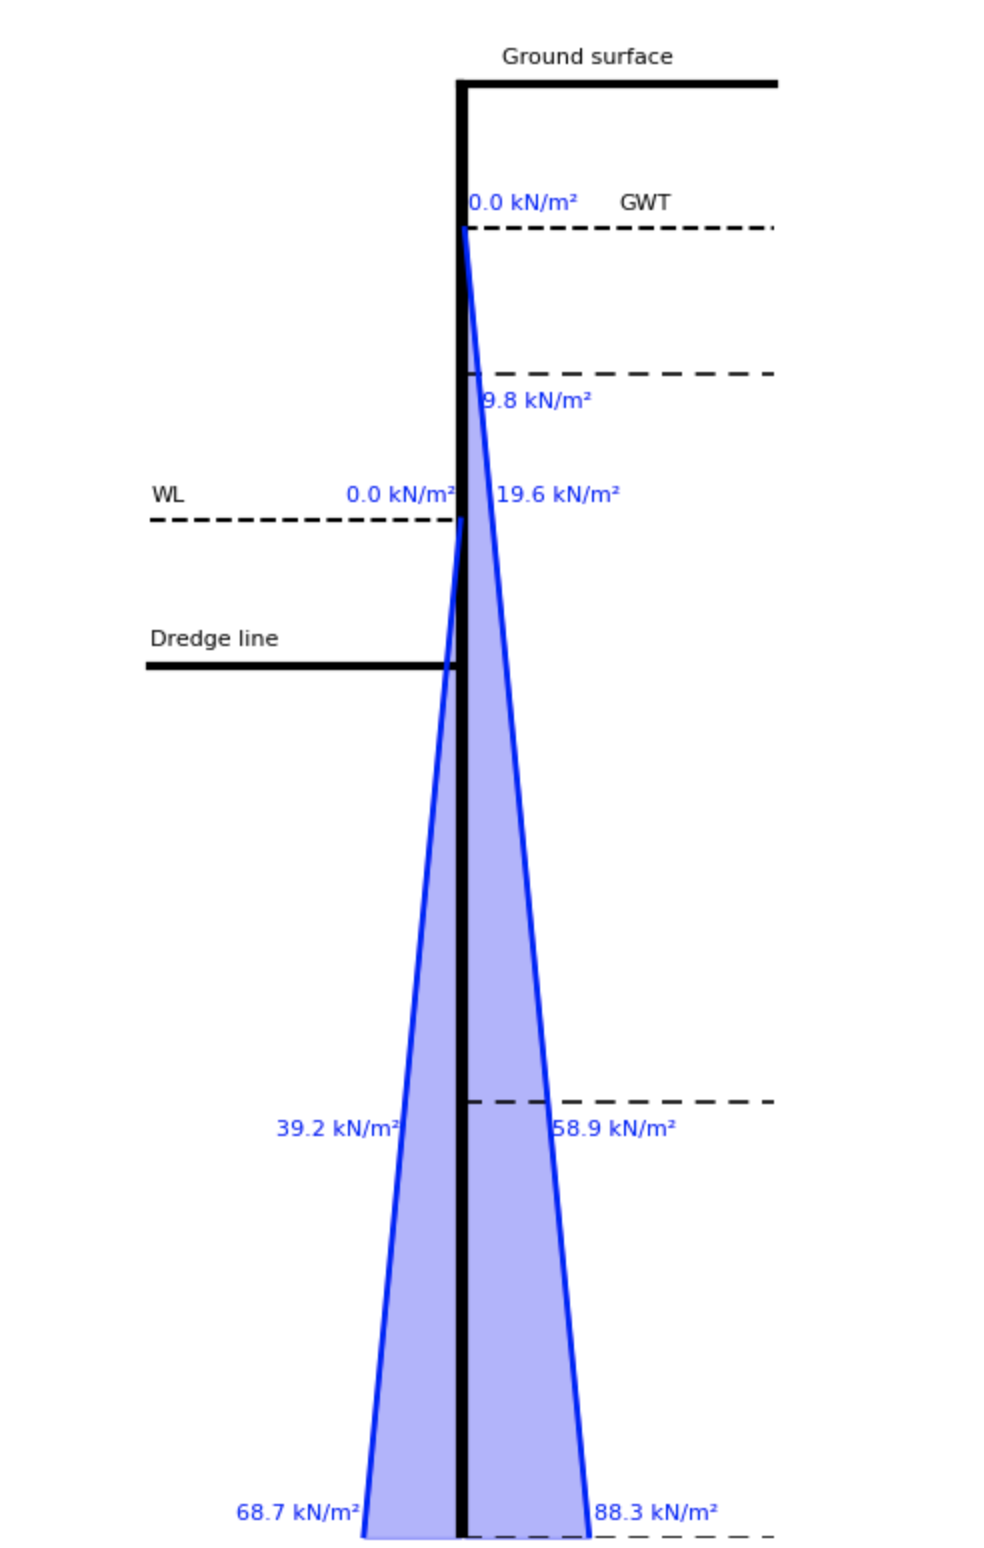
\includegraphics[width=\linewidth, height=10cm]{figures/ch8/water_pressure_small.png}
%         \caption{Hydrostatic pressure}
%         \label{fig:hydrostatic_pressure}
%     \end{subfigure}
%     \hfill
%     \begin{subfigure}[b]{0.45\textwidth}
%         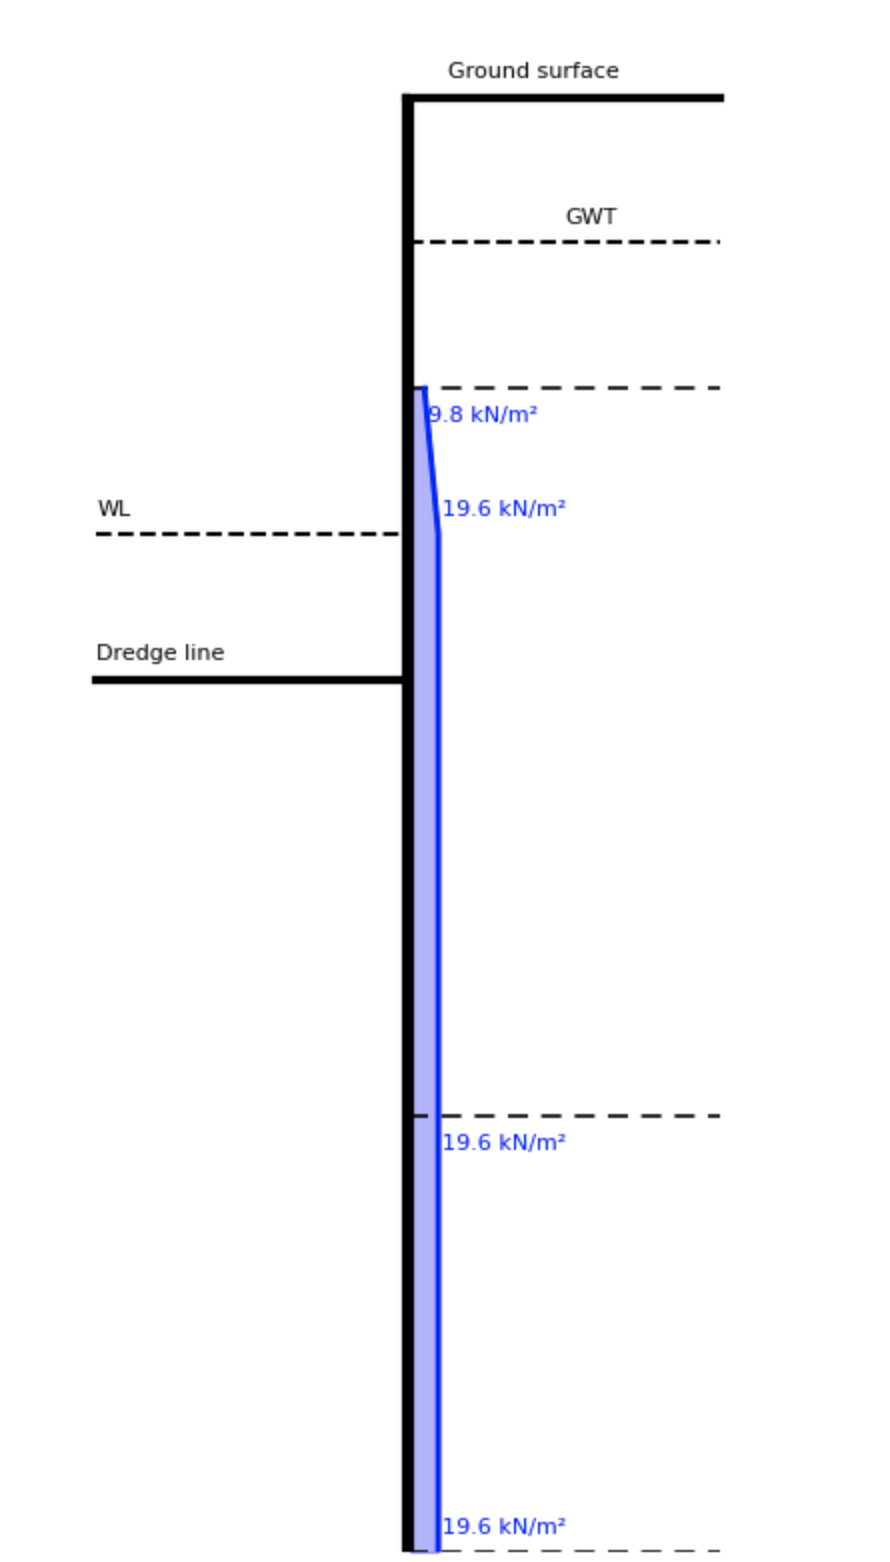
\includegraphics[width=\linewidth, height=10cm]{figures/ch8/excess_water_pressure_small.png}
%         \caption{Excess hydrostatic pressure}
%         \label{fig:excess_hydrostatic_pressure}
%     \end{subfigure}
%     \caption{Excess hydrostatic pressure}
%     \label{fig:excess_pressure}
% \end{figure}

% DEZE PLOT NOG VERBETEREN IN DE CODE EN DUIDELIJKER MAKEN EN DE WAARDES WEGHALEN

% \begin{figure}[H]
%     \centering
%     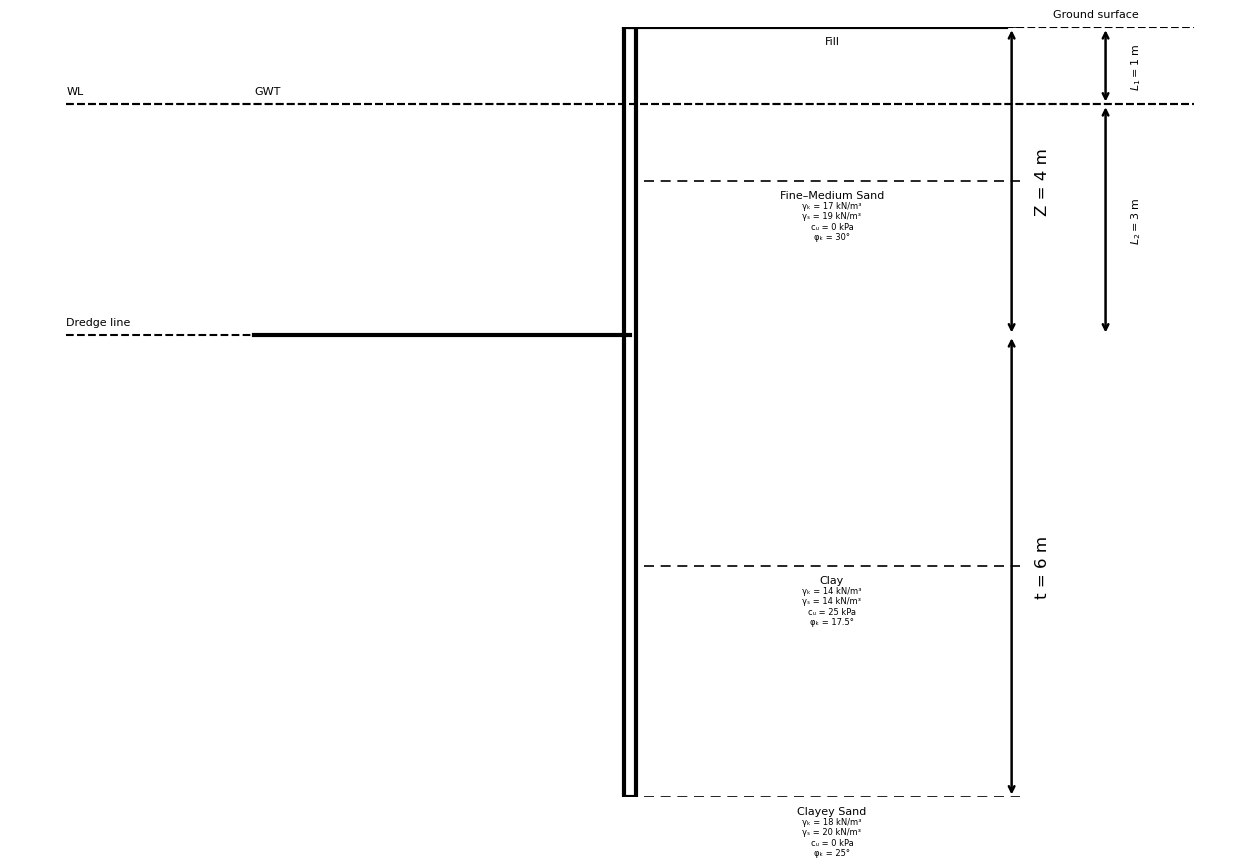
\includegraphics[width=0.70\linewidth]{figures/ch8/soil_profile_cross_section.png}
%     \caption{Soil profile in the cross-section}
%     \label{fig:soil_profile_cross_section}
% \end{figure}

% \subsubsection{ULS and SLS}

% For the calculation for the embedding depth safety factors concerning the ultimate limit state and serviceability limit state should be included. For the calculation, normally, multiple ULS combinations should be calculated and the most unfavorable one is governing. All the combinations are shown in detail in Appendix XX. However, for the following calculation the most unfavorable combination is taken and elaborated.

% HIER BESPREKEN VAN DE VEILIGHEIDSFACTOREN VAN ZOWEL DE KRACHTEN ALS DE GRONDPARAMETERS. OF DIT PAS DOEN BIJ DE VOOR DE BERKENING ZELF. ULS EN SLS BESPREKEN.

\newpage

\section{Design of Steel Sheet Pile}

The design of steel sheet piles begins with defining the design location and problem description to get a better understanding of the situation. After defining these conditions, a method should be considered to calculate the earth pressure and water pressure. These will later balance the moments to iteratively define the embedding depth of the sheet pile wall. After calculating the embedding depth based on the balance of moments, the sheet pile will be verified according to structural verifications, including bending moments, shear force, and deflection.  

To set up the balance of moments for defining the embedding depth, the loads acting on the wall need to be defined. The lateral loads acting on the wall include soil and water pressure, which need to be defined to calculate the forces. The soil parameters are defined, and the soil profile is taken from Section \ref{par:geology}. With the soil profile and its parameters, the earth pressures can be defined on both sides of the sheet pile wall. The hydraulic pressure due to the water levels is of importance, and these are defined in Section \ref{section:hydraulic_parameters}. 

With the problem description defined, a plan to calculate the embedding depth of the sheet pile is set up by using Python code. The plan begins by defining the soil and water parameters, which will be transformed to effective stresses, active and passive earth, and hydrostatic water pressures. From the stresses, the resulting forces acting on the sheet pile wall are defined, and a balance of moments is obtained. Setting the moment to zero at the bottom of the sheet pile wall, the embedding depth is iteratively calculated. The steps for calculating the embedding depth and the structural verification of the sheet pile design are provided in Appendix XX.

% HIER EEN MOOI VERHAAL OVER HOE EEN SHEET PILE WALL DESIGN TOT STAND KOMT. ALGEMEEN VERHAAL VAN HET DESIGN

% BESPREKEN WAT HET PLAN IS OM EEN DESIGN TE MAKEN EN TE BEREKENEN. CUR GEBRUIKEN.

\subsubsection{Location}

The determination of the critical erosion points along the river has been done in Section \ref{section:cirtical_location}. The location analyzed here will be the spot for which the design of the steel sheet pile will be based. In Figure \ref{fig:critical_location}, the critical point is shown in Aqua Monitor, and during the field trip, images were made to verify if the erosion on the Aqua Monitor map was visible. The total length is 215 meters, which is drawn and shown in Table \ref{tab:Surface Lost Camping La Blanqueada in 2022}.

% DEZE TEKST NOG VERBETEREN

\begin{figure}[H]
    \centering
    \begin{subfigure}[b]{0.45\textwidth}
        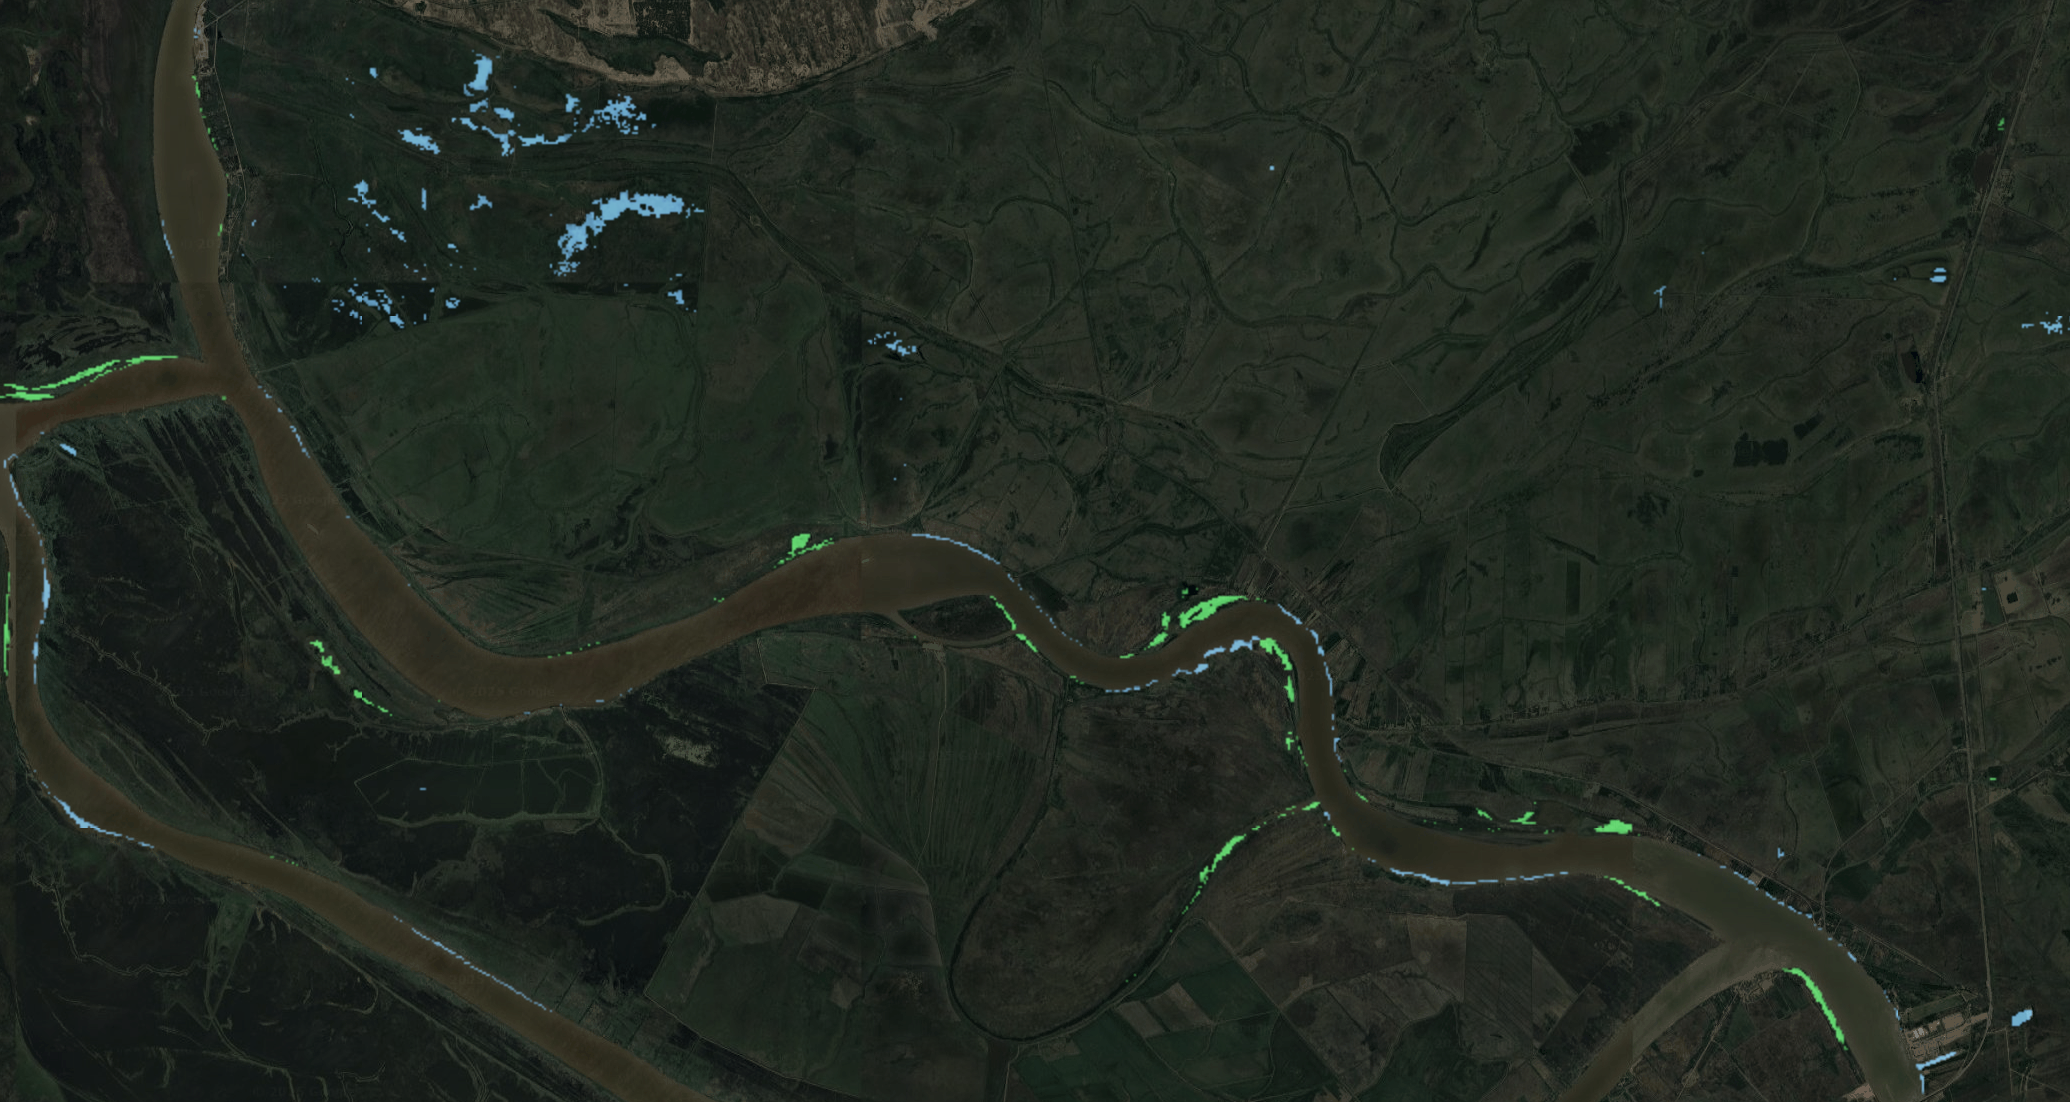
\includegraphics[width=\linewidth, height=5cm]{figures/ch8/critical_location_google.png}
        \caption{Critical location Aqua Monitor}
        \label{fig:critical_location_google}
    \end{subfigure}
    \hfill
    \begin{subfigure}[b]{0.45\textwidth}
        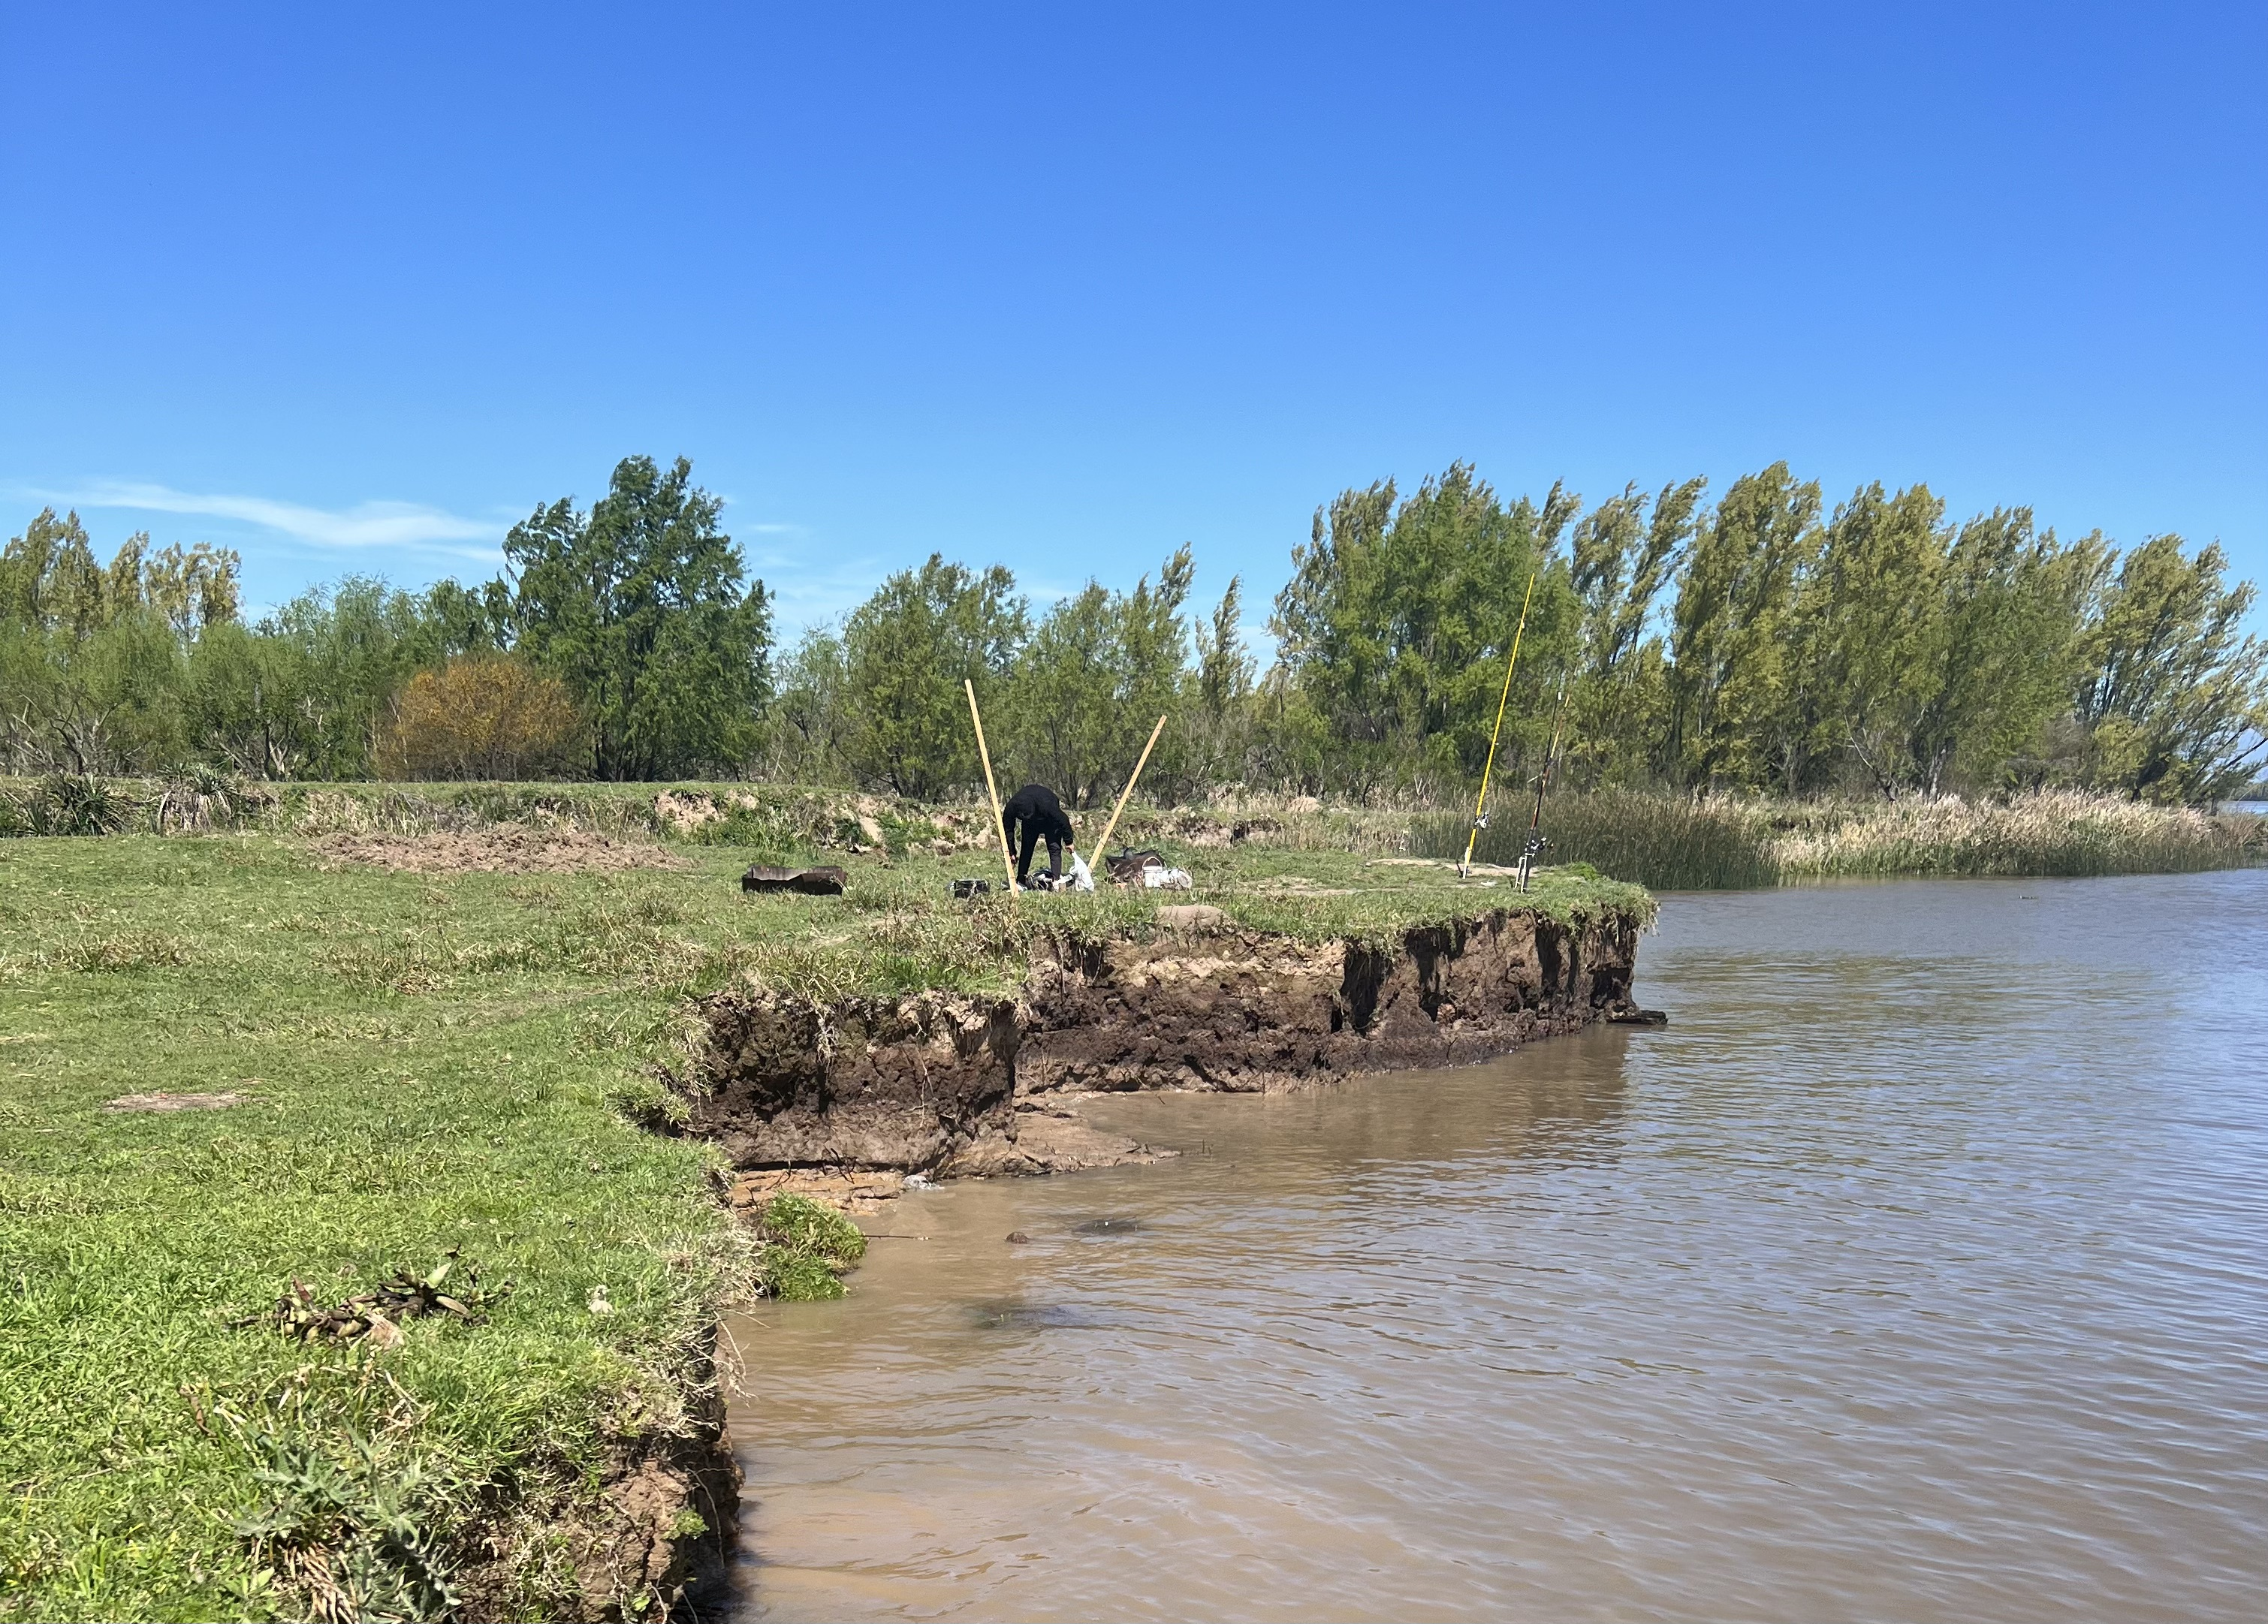
\includegraphics[width=\linewidth, height=5cm]{figures/ch8/critical_location.jpeg}
        \caption{Verification critical point field trip}
        \label{fig:critical_location_fieldtrip}
    \end{subfigure}
    \caption{Critical location}
    \label{fig:critical_location}
\end{figure}

\subsubsection{Geometry of the problem}

The design of the sheet pile wall is based on the cantilever sheet pile wall. As briefly touched on in Section \ref{section:sheet_pile_wall}, the cantilever sheet pile is used for retaining heights up to 5 meters and gets its support from the soil and hydrostatic pressure. In Figure \ref{fig:problem_description_sheetpiles}, a sketch of the situation, made in Python, is provided. The height that needs to be retained, $4.0 \ m$, is indicated with $Z$. The embedment depth of the cantilever sheet pile, which will need to be determined iteratively, is noted as $t$. In this sketch, the groundwater table, $+1.5 \ m \ IGN$, is indicated by the dashed line and the abbreviation $GWT$. The water level of the river is indicated as $WL$, which, in this situation, is $-3.0 \ m$ below the ground surface, $-0.5 \ m \ IGN$. The ground surface, $+2.5 \ m \ IGN$ can seen in the figure, and the levels in comparison to IGN will be explained in Section \ref{section:hydraulic_parameters}. %This will produce the most unfavorable situation and give the largest embedding length for the sheet pile.

% MAKKELIJKER UITLEGGEN HOE HET WERKT. WAT ZIJN DE VERSCHILLENDE NIVEAUS? WELKE HOOGTE MOETEN WE BEPALEN. WELKE ZIJN AL BEPAALD. HOE KOMEN WE AAN DE WATERHOOGTE? HOE KOMEN WE AAN DE GROND WATER STAND?

\begin{figure}[H]
    \centering
    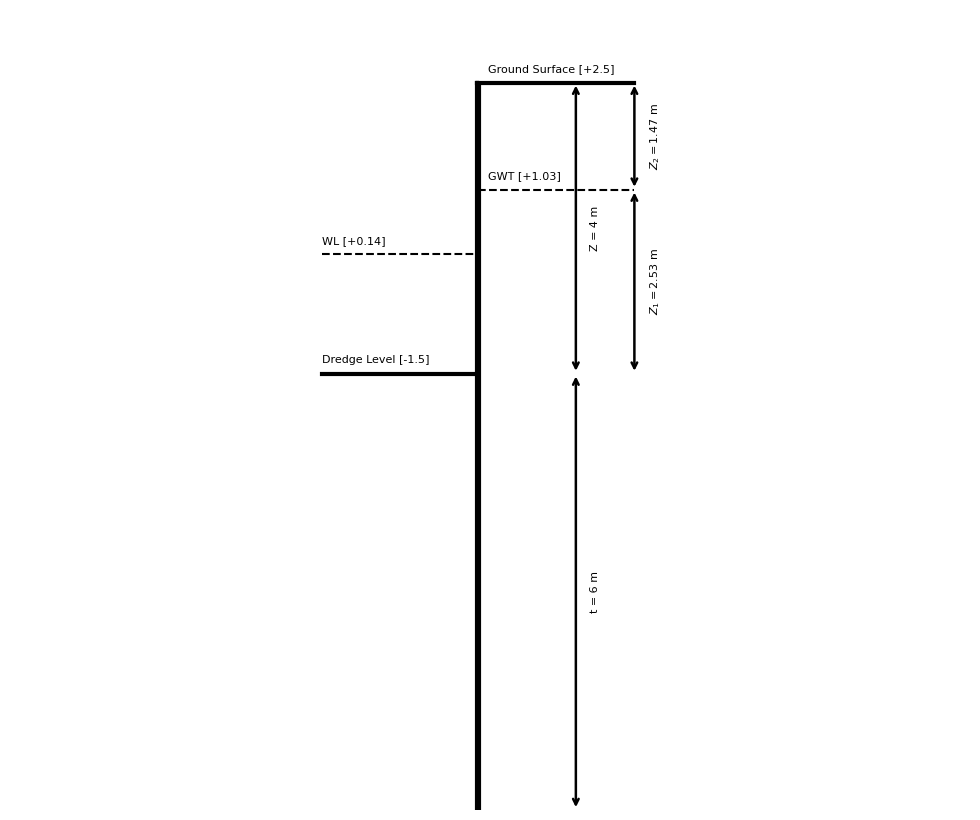
\includegraphics[width=0.90\linewidth]{figures/ch8/cross_section.png}
    \caption{Cross-section for sheet pile}
    \label{fig:problem_description_sheetpiles}
\end{figure}

\begin{itemize}
    \item WL Water level;
    \item GWT Ground water table;
    \item Z Retained height;
    \item t Embedding depth;
    \item $Z_{1}$ Unsaturated soil;
    \item $Z_{2}$ Saturated soil.
\end{itemize}

\subsection{Method}

A design for a cantilever sheet pile can be performed by multiple methods and models. The most common methods that are applicable for sheet pile walls are listed below (Opmaak1):

\begin{itemize}
  \item Bishop;
  \item Pressure bar (push up);
  \item PLAXIS (F.E.M);
  \item Blum-sheet pile wall;
  \item Spring-supported beam;
  \item Terzaghi;
  \item Homberg;
  \item Horizontal balance;
  \item Bakker (PLAXIS);
  \item Piping en heaving.
\end{itemize}

Reviewing Eurocode 7, the calculation for the design of a sheet pile should be based on the spring-supported beam method. However, due to complexity, the sheet pile wall will be calculated using the simplified graphical method of Blum. This method is a simplified representation of the situation, however, after calculating the embedding depth, the verifications will be according to the ultimate limit and serviceability limit defined in Eurocode 3 and Eurocode 7.

\subsubsection{Blum}

The Blum method used for the sheet pile wall is a simplified graphical method, shown in Figure \ref{fig:blum}. The right side of the sheet pile is the "ACTIVE" side, and on the left side, under the dredge level, the "PASSIVE" side. The simplification step in the figure shows an additional resultant force, R, which is acting on the lowest point of the sheet pile. This is done because below this point, the “ACTIVE” and “PASSIVE” sides switch, creating a complex situation. Within the method, a plastic development of the soil and water table level is assumed to be infinitely stiff. To calculate the embedding depth, the sum of moments around the lowest point of the sheet pile wall will be set to zero. The unknown embedding depth can be calculated in multiple ways. In this section, an initial embedding depth will be defined, and iteratively, the moment will be set to zero while increasing or decreasing the embedding depth. However, in this method, no safety factors are taken into account. Therefore, the found embedding depth will have to be increased by $20\%$ (Opmaak1).

\begin{figure}[H]
    \centering
    \begin{subfigure}[b]{0.45\textwidth}
        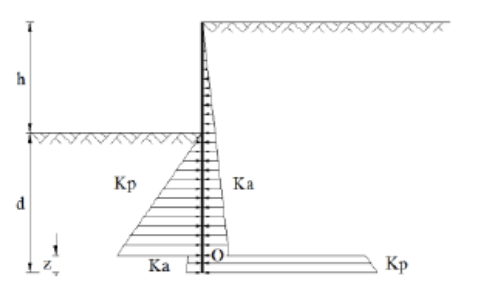
\includegraphics[width=\linewidth, height=5cm]{figures/ch8/blum_1.png}
        \caption{Conventional design}
        \label{fig:conventional_design}
    \end{subfigure}
    \hfill
    \begin{subfigure}[b]{0.45\textwidth}
        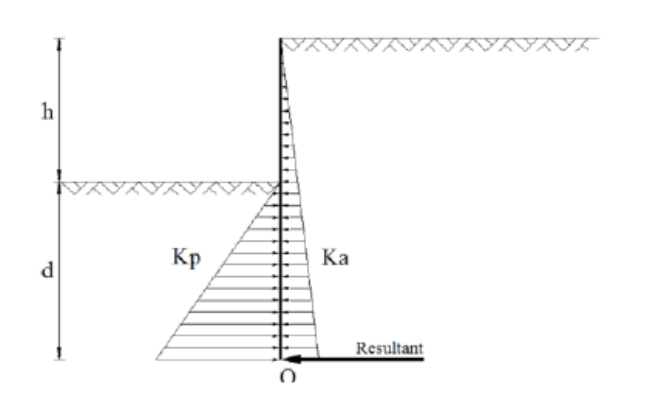
\includegraphics[width=\linewidth, height=5cm]{figures/ch8/blum_2.png}
        \caption{Blum simplification}
        \label{fig:blum_simplification}
    \end{subfigure}
    \caption{Blum simplification method}
    \label{fig:blum}
\end{figure}

% DEZE NOG ZELF MAKEN IN PYTHON OOK EEN DUIDELIJK LOPEND VERHAAL MAKEN. BLUM VEREENVOUDIGD. WAAROM MAG DAT? WAAR MOETEN WE OP BLIJVEN LETTEN IN HET VERDERE ONTWERPPROCES?

% \begin{figure}[H]
%     \centering
%     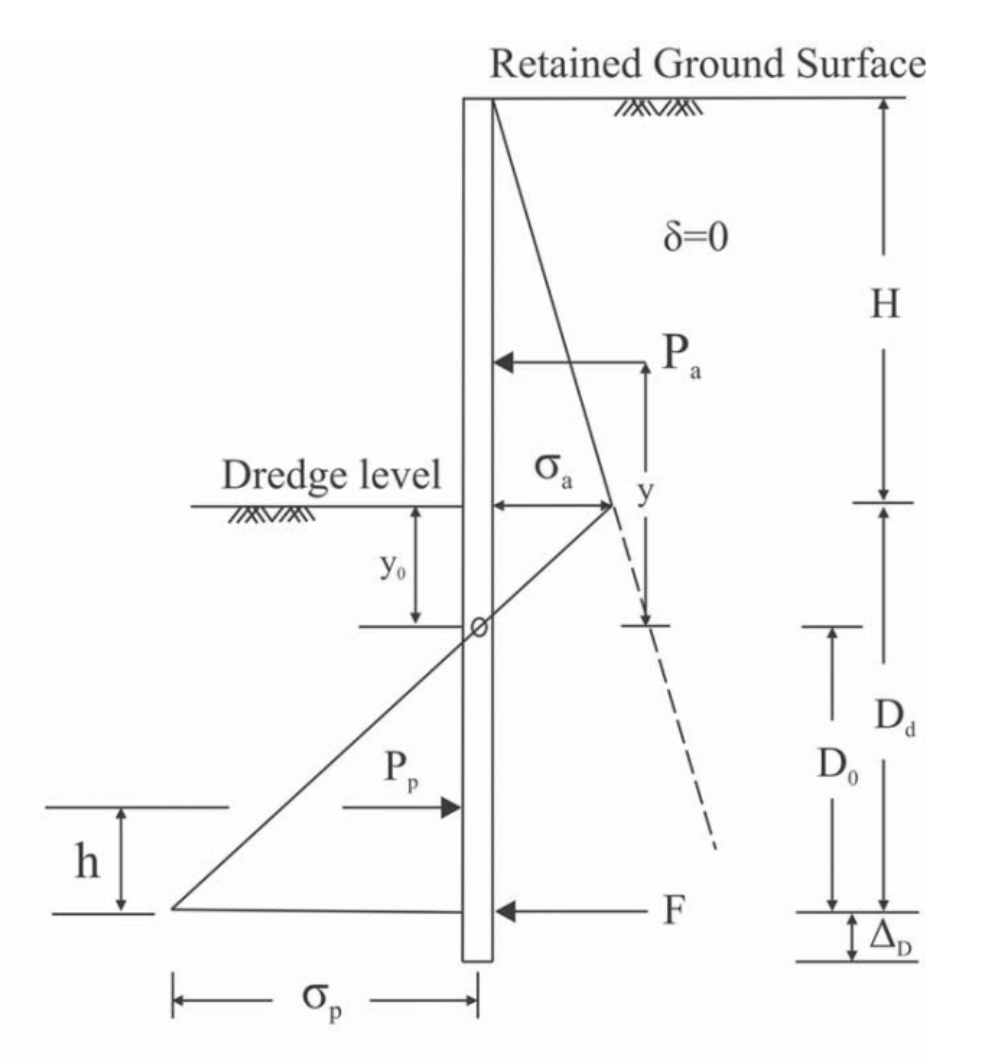
\includegraphics[width=0.70\linewidth]{figures/ch8/blum_methode.png}
%     \caption{Blum method}
%     \label{fig:blum_method}
% \end{figure}

\subsection{Embedding depth}

The embedding depth of the sheet pile is derived from the balance of moment around the lowest point. The balance of moments should be set to zero, providing the minimal embedding depth. To make up the balance of moments, the pressures acting on the sheet pile should be defined to transform these into forces. The horizontal pressure acting on the sheet pile is the earth and hydrostatic pressure. First, the earth pressures will be analyzed by the Python code. Hereafter, the hydrostatic analysis will be performed, and the forces will be calculated. 

The depth can be defined in multiple ways. A method is to keep the depth as an unknown parameter, $t$. This will provide an explicit formula for moving below the dredge line, for the pressure and resulting forces. As the forces will be related to the balance of moments, roots will be held to get the unknown $t$. However, another approach is to begin with an estimated depth and calculate the sum of moments around the lowest point. As this balance will not be zero, an iterative solution can be used to make sure the depth is increasing while optimizing the moment balance to zero at the lowest part of the sheet pile. In this design, the depth of the sheet pile is based on the second approach. The first value of the embedding depth is taken as $6.0$ meters, which can be seen in Figure \ref{fig:problem_description_sheetpiles}.

\newpage

\subsubsection{Vertical effective stress}

The horizontal pressure of the soil can be calculated based on the effective stress. The effective stress in the soil can be calculated with Equation \ref{eq:effective_stress}. The stress is based on the height of the soil and the unit weight $\gamma$, of each layer. If the soil layer is below the groundwater table, the saturated unit weight should be deducted from the unit weight, $\gamma - \gamma_{w}$. In Figure \ref{eq:effective_stress}, the effective stress on both sides of the sheet pile can be seen, and the corresponding values are provided in Table XX.

\begin{equation}
    \sigma^{'}_{z} = z \cdot \gamma
    \label{eq:effective_stress}
\end{equation}

\begin{figure}[H]
    \centering
    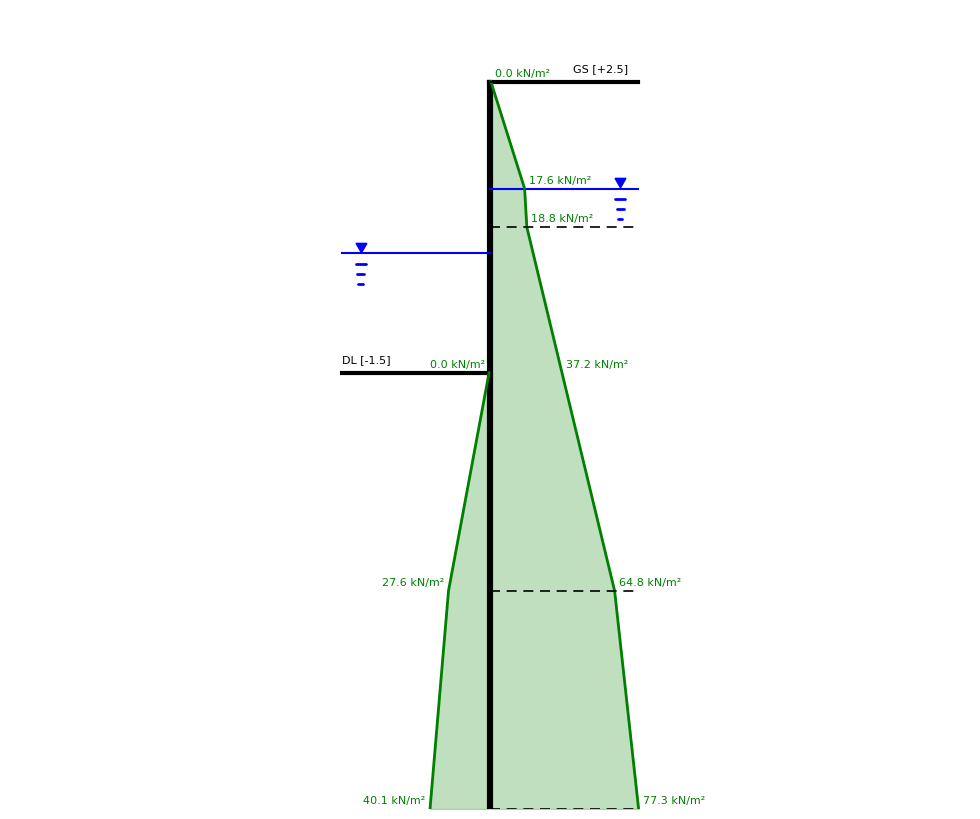
\includegraphics[width=0.7\linewidth]{figures/ch8/effective_stress.png}
    \caption{Effective stress "ACTIVE" and "PASSIVE" side}
    \label{fig:effective_stress}
\end{figure}

% \begin{table}[ht]
%   \centering
%   \caption{Vertical effective stress on left and right sides}
%   \label{tab:effective_stress}
%   \small
%   \setlength{\tabcolsep}{8pt}
%   \renewcommand{\arraystretch}{1.15}
%   \begin{tabular}{@{}r r r@{}}
%     \toprule
%     $z$ [m] &
%     $\sigma'_{z,l}$ [kN/m$^2$] &
%     $\sigma'_{z,r}$ [kN/m$^2$] \\
%     \midrule
%      0.00 &  0.00 &  0.00 \\
%      1.00 &  0.00 & 12.00 \\
%      2.00 &  0.00 & 14.19 \\
%      4.00 &  0.00 & 32.57 \\
%      7.00 & 27.57 & 60.14 \\
%     10.00 & 40.14 & 72.71 \\
%     \bottomrule
%   \end{tabular}
% \end{table}

\subsubsection{Earth pressure and force}

The pressure the wall feels from the soil is the lateral earth pressure. This earth pressure can be calculated with the effective vertical stress and a coefficient. While soil is largely dependent on nature, the stresses differ, just like the vertical effective stress along the profile. Equation \ref{eq:earth_pressure} shows how the earth pressures are calculated for both the “ACTIVE” and “PASSIVE” sides. For the “ACTIVE” and “PASSIVE” sides, the coefficients $K_{a}$ and $K_{p}$ will be used.

\begin{equation}
    p_{ea,h,z} = z \cdot \gamma \cdot K_{\gamma}
    \label{eq:earth_pressure}
\end{equation}

The "ACTIVE" and "PASSIVE" earth coefficients can be computed by Equations \ref{eq:K_gamma_a_k} and \ref{eq:K_gamma_p_k}. These equations are regarding the Coulomb theory and in this calculation the $\alpha$, $\beta$, and $\delta$, which are the slope of the sheet pile, slope of the ground levels, and wall friction angle are equal to zero. Therefore, Equations \ref{eq:Ka_tan} and \ref{eq:Kp_tan} are used.

\begin{equation}
    K_{\gamma;a;k} =
    \frac{
        \cos^{2}\!\left(\varphi' + \alpha\right)
    }{
        \cos^{2}(\alpha)
        \left(
            1 +
            \sqrt{
                \frac{
                    \sin\!\left(\varphi' + \delta_{a;k}\right)
                    \sin\!\left(\varphi' - \beta_a\right)
                }{
                    \cos\!\left(\alpha - \delta_{a;k}\right)
                    \cos\!\left(\alpha + \beta_a\right)
                }
            }
        \right)^{2}
    }
    \label{eq:K_gamma_a_k}
\end{equation}

\begin{equation}
    K_{\gamma;p;k} =
    \frac{
        \cos^{2}\!\left(\varphi' - \alpha\right)
    }{
        \cos^{2}(\alpha)
        \left(
            1 -
            \sqrt{
                \frac{
                    \sin\!\left(\varphi' - \delta_{p;rep}\right)
                    \sin\!\left(\varphi' + \beta_p\right)
                }{
                    \cos\!\left(\alpha - \delta_{p;k}\right)
                    \cos\!\left(\alpha + \beta_p\right)
                }
            }
        \right)^{2}
    }
    \label{eq:K_gamma_p_k}
\end{equation}

\begin{equation}
    K_{\gamma,a} = \tan^{2}\!\left(45^\circ - \frac{\varphi'}{2}\right)
    \label{eq:Ka_tan}
\end{equation}

\begin{equation}
    K_{\gamma,p} = \tan^{2}\!\left(45^\circ + \frac{\varphi'}{2}\right)
    \label{eq:Kp_tan}
\end{equation}

Using Table \ref{tab:soil_layers}, in which all soil parameters are included, the effective angle of internal friction is needed to calculate the “ACTIVE” and “PASSIVE” coefficients for the different layers. Table \ref{tab:layers_ka_kp} gives an overview of the “ACTIVE” and “PASSIVE” coefficients for the different layers. 

\begin{table}[H]
  \centering
  \caption{Soil layers and earth pressure coefficients.}
  \label{tab:layers_ka_kp}
  \small
  \setlength{\tabcolsep}{8pt}
  \renewcommand{\arraystretch}{1.15}
  \begin{tabular}{@{}r l l r r r@{}}
    \toprule
    Layer & Soil type & Depth [m] &
    $\varphi'\,[\boldsymbol{^\circ}]$ &
    $K_{\gamma,a}$ [-] & $K_{\gamma,p}$ [-] \\
    \midrule
    1 & Fill             & 0.0 - 2.0   & 15.0 & 0.589 & - \\
    2 & Fine--Medium Sand& 2.0 - 7.0   & 30.0 & 0.333 & 3.000 \\
    3 & Clay             & 7.0 - 10.0  & 17.5 & 0.538 & 1.860 \\
    4 & Clayey Sand      & 10.0 - 15.0 & 25.0 & 0.406 & 2.464 \\
    \bottomrule 
  \end{tabular}
\end{table}

Figure \ref{fig:earth_pressure} shows an overview of the “ACTIVE” and “PASSIVE” earth pressure acting on the wall. When calculating the earth pressures, it should be noted that for the interfaces of the soil layers, the rightful coefficient is taken and multiplied with the effective stress, $\sigma_{z}$. From the “ACTIVE” and “PASSIVE” pressure acting on the sheet pile, one can determine the horizontal forces. The horizontal force is calculated with Equation \ref{eq:earth_force} within Python, where the “ACTIVE” and “PASSIVE” earth pressure is multiplied by the height of its layer. For triangular shapes, the Equation \ref{eq:earth_force} should be multiplied by a factor of $\frac{1}{2}$.

For the force magnitude, triangles and rectangles were computed by Python, and the corresponding forces were defined. In Figure \ref{fig:earth_pressure}, an overview of all the forces is shown. An overview of the segments, corresponding values, and point of application is shown in Table XX.

\begin{equation}
    F_{ea,h,z} = p_{ea,h,z} \cdot h_{layer}
    \label{eq:earth_force}
\end{equation}

\begin{figure}[H]
    \centering
    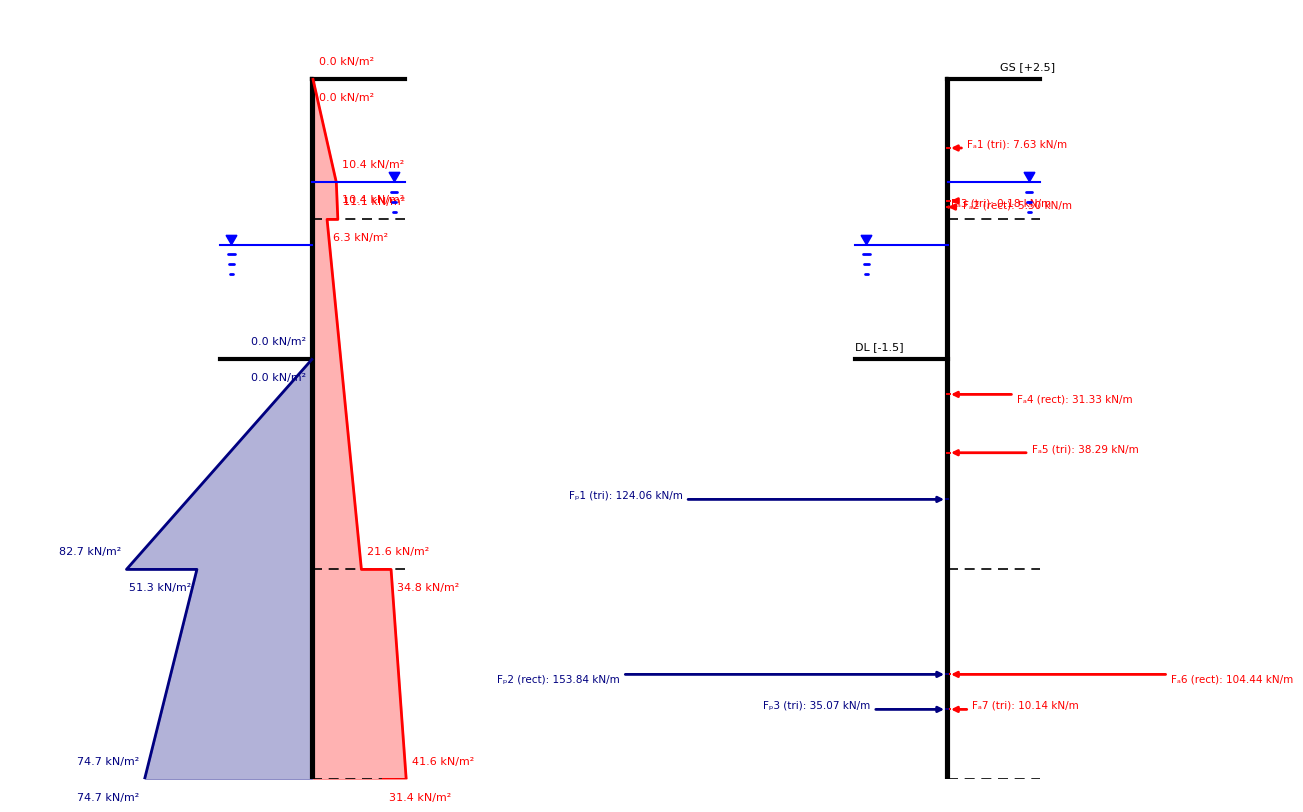
\includegraphics[width=0.75\linewidth]{figures/ch8/earth_pressure_force.png}
    \caption{Earth pressure (left) and force (right)}
    \label{fig:earth_pressure}
\end{figure}


% \begin{table}[ht]
%   \centering
%   \caption{Active and passive pressures}
%   \label{tab:earth_pressure_values}
%   \small
%   \setlength{\tabcolsep}{6pt}
%   \renewcommand{\arraystretch}{1.15}
%   \begin{tabular}{@{}r r r r r@{}}
%     \toprule
%     $z$ [m] &
%     $p_{above, passive}$ [kN/m$^2$] &
%     $p_{below, passive}$ [kN/m$^2$] &
%     $p_{above, active}$ [kN/m$^2$] &
%     $p_{below, active}$ [kN/m$^2$] \\
%     \midrule
%      0.00 & \textemdash & \textemdash &  0.00 &  0.00 \\
%      1.00 & \textemdash & \textemdash &  7.07 &  7.07 \\
%      2.00 & \textemdash & \textemdash &  8.35 &  4.73 \\
%      4.00 &  0.00 &  0.00 & \textemdash & \textemdash \\
%      7.00 & 82.71 & 51.28 & 20.05 & 32.33 \\
%     10.0 & 74.66 & 74.66 & 39.09 & 29.51 \\
%     \bottomrule
%   \end{tabular}
% \end{table}

% \begin{table}[H]
%   \centering
%   \caption{Resultant forces and centroids by segment.}
%   \label{tab:forces_centroids}
%   \small
%   \setlength{\tabcolsep}{8pt}
%   \renewcommand{\arraystretch}{1.15}
%   \begin{tabular}{@{}l r l r r@{}}
%     \toprule
%     Side & Segment & Shape &
%     F [kN/m] & $z_c$ [m] \\
%     \midrule
%     Active & 1 & Triangle  &  3.53 & 0.67 \\
%     Active & 2 & Rectangle &  7.07 & 1.50 \\
%     Active & 2 & Triangle  &  0.64 & 1.67 \\
%     Active & 3 & Rectangle & 23.65 & 4.50 \\
%     Active & 3 & Triangle  & 38.29 & 5.33 \\
%     Active & 4 & Rectangle & 97.00 & 8.50 \\
%     Active & 4 & Triangle  & 10.14 & 9.00 \\
%     Passive & 1 & Triangle  & 124.06 & 6.00 \\
%     Passive & 2 & Rectangle & 153.84 & 8.50 \\
%     Passive & 2 & Triangle  &  35.07 & 9.00 \\
%     \bottomrule
%   \end{tabular}
% \end{table}

\newpage

\subsubsection{Hydrostatic pressure and force}

The hydrostatic pressure $w$ is referred to as the pore water pressure. In unconfined groundwater, the pore water pressure at a depth z is calculated by Equation \ref{eq:pore_water_pressure}.

\begin{equation}
    w = z \cdot \gamma_{w}
    \label{eq:pore_water_pressure}
\end{equation}

When there is an excess of hydrostatic pressure, meaning that the water levels on both sides of the wall are not at the same level, an excess hydrostatic pressure will occur. The excess hydrostatic pressure can be calculated with Equation \ref{eq:excess_water_pressure}. In Figure \ref{fig:hydrostatic_excess_pressure}, an overview of the hydrostatic water pressure and force is given.

\begin{equation}
    w_{u}(z) = w_{r}(z) - w_{l}(z) = h_{r}(z) \cdot \gamma_{w} - h_{l}(z) \cdot \gamma_{w}
    \label{eq:excess_water_pressure}
\end{equation}

\begin{figure}[H]
    \centering
    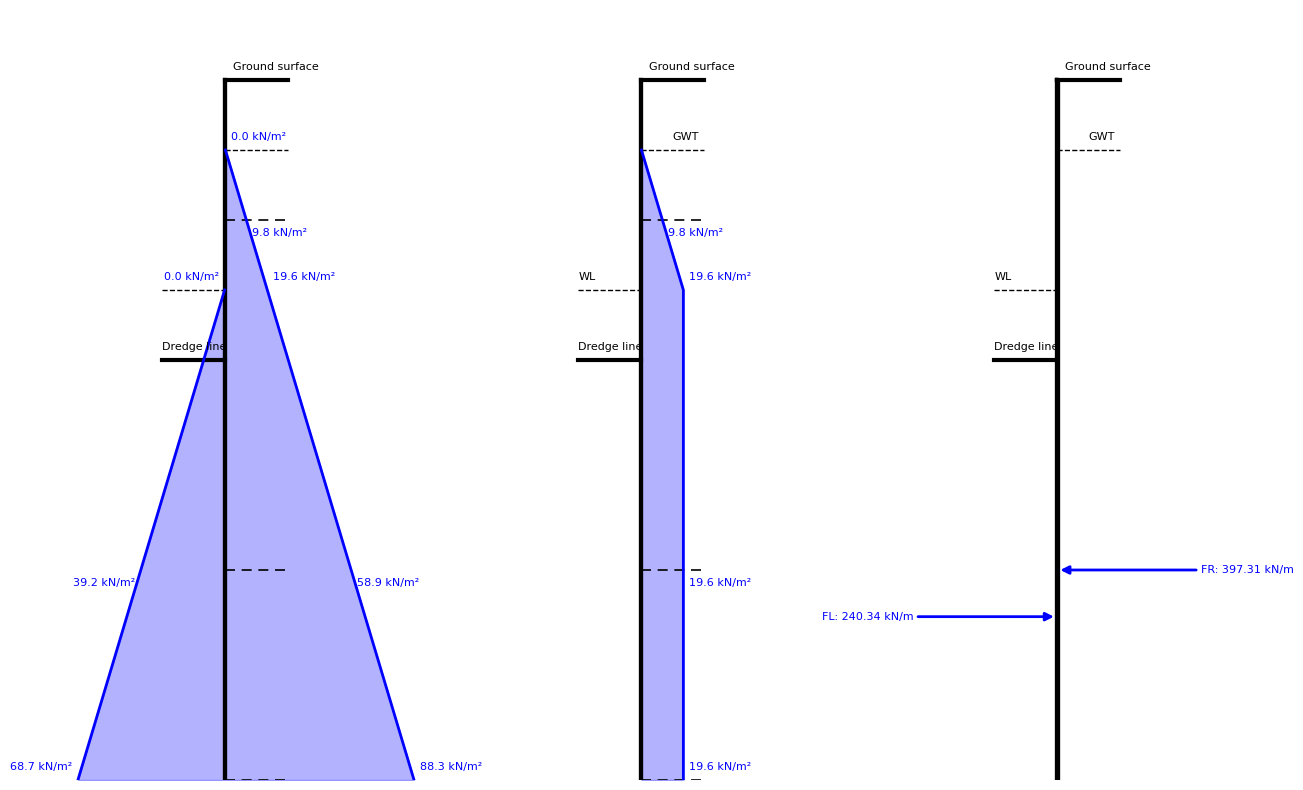
\includegraphics[width=0.75\linewidth]{figures/ch8/water_overview.png}
    \caption{Hydrostatic pressure (right), excess hydrostatic pressure (center), and forces (right)}
    \label{fig:hydrostatic_excess_pressure}
\end{figure}

% \begin{table}[ht]
%   \centering
%   \caption{Pore pressure values along depth.}
%   \label{tab:u_profile}
%   \small
%   \setlength{\tabcolsep}{8pt}
%   \renewcommand{\arraystretch}{1.15}
%   \begin{tabular}{@{}l l l l@{}}
%     \toprule
%     \textbf{$z$ [m]} &
%     \textbf{$u_{right}$ [kN/m$^2$]} &
%     \textbf{$u_{left}$ [kN/m$^2$]} &
%     \textbf{$u_{net}$ [kN/m$^2$]} \\
%     \midrule
%      0.00  &  0.00  &  0.00  &  0.00 \\
%      1.00  &  0.00  &  0.00  &  0.00 \\
%      2.00  &  9.81  &  0.00  &  9.81 \\
%      3.00  & 19.62  &  0.00  & 19.62 \\
%      7.00  & 58.86  & 39.24  & 19.62 \\
%     10.00  & 88.29  & 68.67  & 19.62 \\
%     \bottomrule
%   \end{tabular}
% \end{table}

% \textit{Balance of Forces}

% \begin{equation}
%     \sum{F_{H}} = 0
%     \label{eq:balance_forces}
% \end{equation}

\subsubsection{Bending moment}

The balance of moments around the lowest part of the sheet pile should be zero,  stated in Equation \ref{eq:moment}. For $t = 6.0 \ m$, in Figure XX, this point, "O", is indicated, and the forces acting due to both the earth and the hydrostatic pressure are shown. From the acting forces and the distance to point "O", the moments are computed. In Table XX, it can be seen that the balance of moments, for $t = 6.0 \ m$, is not equal to zero, but $156.3 \ kNm/m$. Indicating an iterative calculation, increasing the embedding depth, and checking at which depth the moments are equal to zero, is required.

\begin{equation}
    \sum{M_{t}} = 0
    \label{eq:moment}
\end{equation}

 After an iteration process, in Python, the embedding depth is set to $7.574 \ m$. In Figure \ref{fig:final_moments_balance}, the forces related to this depth are shown. In Table \ref{tab:forces_arms_moments_9713}, the values of the forces and moments are shown, and the resulting moment around the point "O" is close to zero, $0.0512 \ kNm/m$. Regarding the safety factor, the Blum method says that the depth of embedding found should be increased by $20\%$, giving the following depth:

\begin{equation}
    t_{blum} = 1.20 \cdot 7.574 = 9.09 \ m
\end{equation}

\begin{figure}[H]
    \centering
    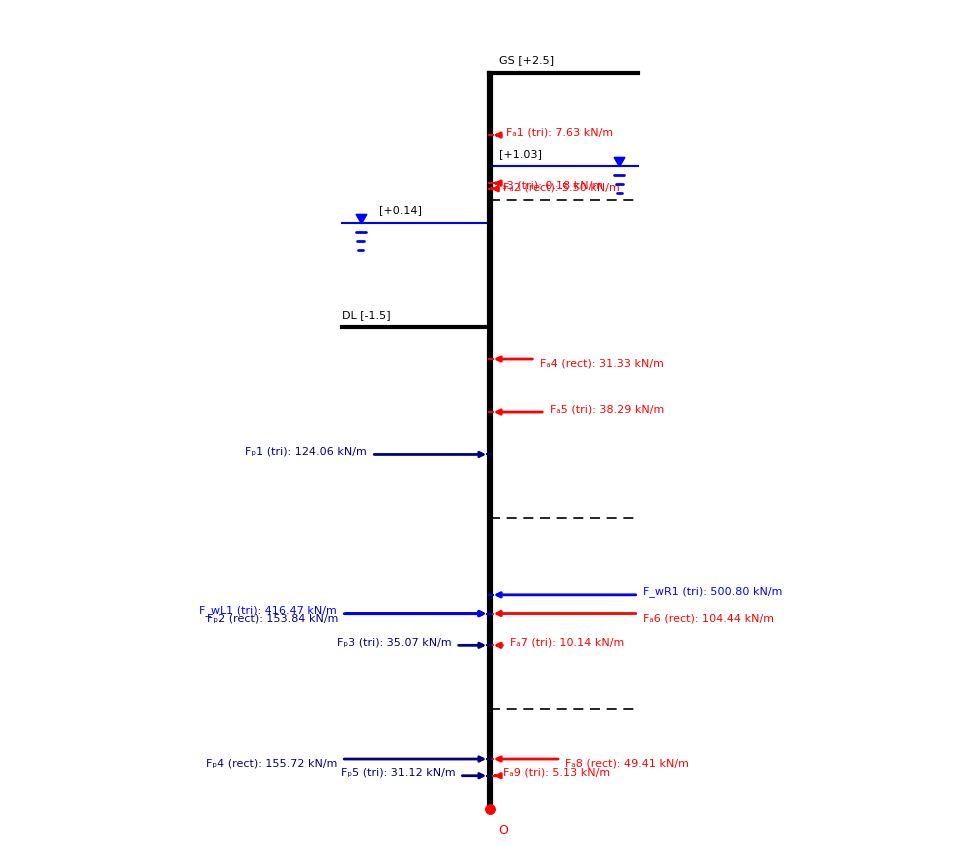
\includegraphics[width=0.90\linewidth]{figures/ch8/moment_balance_7574.png}
    \caption{Forces for $t = 7.574 \ m$}
    \label{fig:final_moments_balance}
\end{figure}

% DEZE NOG AANPASSEN NAAR DE JUISTE SCHAAL RECHTS.

% \begin{table}[H]
%   \centering
%   \caption{Resultant forces, arms, and moments for $t = 6.0$ meters}
%   \label{tab:forces_arms_moments_now}
%   \small
%   \setlength{\tabcolsep}{8pt}
%   \renewcommand{\arraystretch}{1.15}
%   \begin{tabular}{@{}l l r r r@{}}
%     \toprule
%     Side & Shape &
%     F [kN/m] & $z_{base}$[m] &
%     $M_{\text{base}}$ [kN$\cdot$m/m] \\
%     \midrule
%     ACTIVE & Triangle  &  7.63  & 9.02 &  68.86 \\
%     ACTIVE & Rectangle &  5.50  & 8.27 &  45.50 \\
%     ACTIVE & Triangle  &  0.18  & 8.18 &   1.48 \\
%     ACTIVE & Rectangle & 31.33  & 5.50 & 172.34 \\
%     ACTIVE & Triangle  & 38.29  & 4.67 & 178.69 \\
%     ACTIVE & Rectangle & 104.44  & 1.50 & 156.65 \\
%     ACTIVE & Triangle  & 10.14  & 1.00 &  10.14 \\
%     HYDRO PASSIVE & Triangle  & 286.30  & 2.55 &  -730.07 \\
%     HYDRO ACTIVE & Triangle  & 356.89  & 2.84 &  1014.8 \\
%     PASSIVE & Triangle  & 124.06 & 4.00 & -496.26 \\
%     PASSIVE & Rectangle & 153.84 & 1.50 & -230.76 \\
%     PASSIVE & Triangle  &  35.07 & 1.00 &  -35.07 \\
%     \midrule
%     $\sum{M_{t}}$ (should ≈ 0 for equilibrium) &  &  & & 156.3 \\
%     \bottomrule
%   \end{tabular}
% \end{table}

% NAAR BIJLAGE

\begin{table}[H]
  \centering
  \caption{Resultant forces, arms, and moments for $t = 7.574$ meters}
  \label{tab:forces_arms_moments_9713}
  \small
  \setlength{\tabcolsep}{8pt}
  \renewcommand{\arraystretch}{1.15}
  \begin{tabular}{@{}l l r r r@{}}
    \toprule
    Side & Shape &
    F [kN/m] & $z_{base}$ [m] &
    $M_{\text{base}}$ [kN$\cdot$m/m] \\
    \midrule
    ACTIVE  & Triangle  &   7.63  & 10.59 &  80.88 \\
    ACTIVE  & Rectangle &   5.50  &  9.84 &  54.16 \\
    ACTIVE  & Triangle  &   0.18  &  9.75 &   1.77 \\
    ACTIVE  & Rectangle &  31.33  &  7.07 & 221.67 \\
    ACTIVE  & Triangle  &  38.29  &  6.24 & 238.98 \\
    ACTIVE  & Rectangle & 104.44  &  3.07 & 321.08 \\
    ACTIVE  & Triangle  &  10.14  &  2.57 &  26.10 \\
    ACTIVE  & Rectangle &  49.41  &  0.79 &  38.90 \\
    ACTIVE  & Triangle  &   5.13  &  0.52 &   2.69 \\
    HYDRO PASSIVE   & Triangle  & 416.47  &  3.07 & -1279.17 \\
    HYDRO ACTIVE    & Triangle  & 500.80  &  3.37 & 1686.78 \\
    PASSIVE & Triangle  & 124.06  &  5.57 &  -691.60 \\
    PASSIVE & Rectangle & 153.84  &  3.07 &  -472.98 \\
    PASSIVE & Triangle  &  35.07  &  2.57 &   -90.29 \\
    PASSIVE & Rectangle & 155.72  &  0.79 &  -122.59 \\
    PASSIVE & Triangle  &  31.12  &  0.52 &   -16.33 \\
    \midrule
    $\sum M_{t}$ (should ≈ 0 for equilibrium) & & & & 0.0512 \\
    \bottomrule
  \end{tabular}
\end{table}

% HIER EEN PLOT MET DE SOM VAN DE MOMENTEN OM HET LAAGSTE PUNT BIJ EEN GEKOZEN DIEPTE. HIERNA EEN TABEL MET DE WAARDES EN DAT DE MOMENTSOM NIET GELIJK IS AAN NUL.

% HIER EEN PLOT MET HET ITERATIEF BEPALEN VAN DIEPTE WANNEER DE MOMENTENSOM GELIJK IS AAN NUL. VERWIJZEN NAAR DE TABEL IN DE BIJLAGE EN ALLEEN HET RESULTAAT LATEN ZIEN. OOK WELLICHT DE PLOT VAN HANDBOOK OVERNEMEN.

\subsubsection{ULS and SLS}

A cantilever sheet pile wall should be designed according to two conditions. These conditions are the Ultimate Limit State (ULS) and the Serviceability Limit State (SLS). In the ULS, the worst possible forces that can occur during the span of the sheet pile should be analyzed with respect to the safety of people and the structure. In the SLS checking the structure under normal conditions where the function and appearance of the structure are concerned.

For the design, this means that safety factors for the ULS and SLS should be included, regarding Eurocode 7, which is not included with the Blum method. For the analysis, multiple combinations should be verified, and the most unfavorable is used for the design. Two combinations, within design approach 1, stated in Eurocode 7, are evaluated in Appendix XX. However, for the calculation in this section, the most unfavorable combination is taken and elaborated.

The most unfavorable combination within design approach 1 is combination 2 (DA1-2). The safety factors are shown in Table \ref{tab:partial_factors}, and the partial factors on loads, materials, and actions to protect the sheet pile in ULS are shown. In this calculation, the hydrostatic loads and the earth pressures are permanent. For the SLS, all safety factors are set at 1.0. The combination and safety factors result in the final embedding depth of $t = 10.172$ meters,  shown in Figure XX. However, the acting shear forces and bending moments are greater. From Table XX, it can be seen that the balance of moments at this depth is close to zero ($-0.0632 \ kNm/m$).

% WATER PERMANENT VERANDEREN IN BEREKENING.

\begin{equation}
    t_{uls} = 10.172 \ m
\end{equation}

\begin{table}[H]
\centering
\small
\setlength{\tabcolsep}{8pt}
\renewcommand{\arraystretch}{1.2}
\begin{tabular}{@{}l l l c c@{}}
\toprule
\multicolumn{1}{l}{Parameter} & 
\multicolumn{1}{l}{ } & 
\multicolumn{1}{l}{Partial factor} & 
\multicolumn{2}{c}{Combination}\\
\cmidrule(lr){4-5}
 & & & 1 & 2 \\
\midrule
\multirow{4}{*}{\textit{Actions}} 
 & Permanent, Unfavourable & $\gamma_G$ & 1.35 & 1.00 \\
 & Permanent, Favourable   & $\gamma_{G,\mathrm{fav}}$ & 1.00 & 1.00 \\
 & Variable, Unfavourable  & $\gamma_Q$ & 1.50 & 1.30 \\
 & Variable, Favourable\textsuperscript{1)} & -- & 0 & 0 \\
\midrule
\multirow{5}{*}{\textit{Material properties}} 
 & Effective shearing resistance & $\gamma_\varphi$ & 1.00 & 1.25 \\
 & Effective cohesion & $\gamma_c$ & 1.00 & 1.25 \\
 & Undrained shear strength & $\gamma_{cu}$ & 1.00 & 1.40 \\
 & Unconfined compressive strength & $\gamma_{qu}$ & 1.00 & 1.40 \\
 & Weight density & $\gamma_\gamma$ & 1.00 & 1.00 \\
\midrule
\textit{Earth resistance} & & $\gamma_{Re}$ & 1.00 & 1.00 \\
\bottomrule
\end{tabular}
\caption{Partial factors for actions, material properties, and earth resistance.}
\label{tab:partial_factors}
\end{table}

% \begin{figure}[H]
%     \centering
%     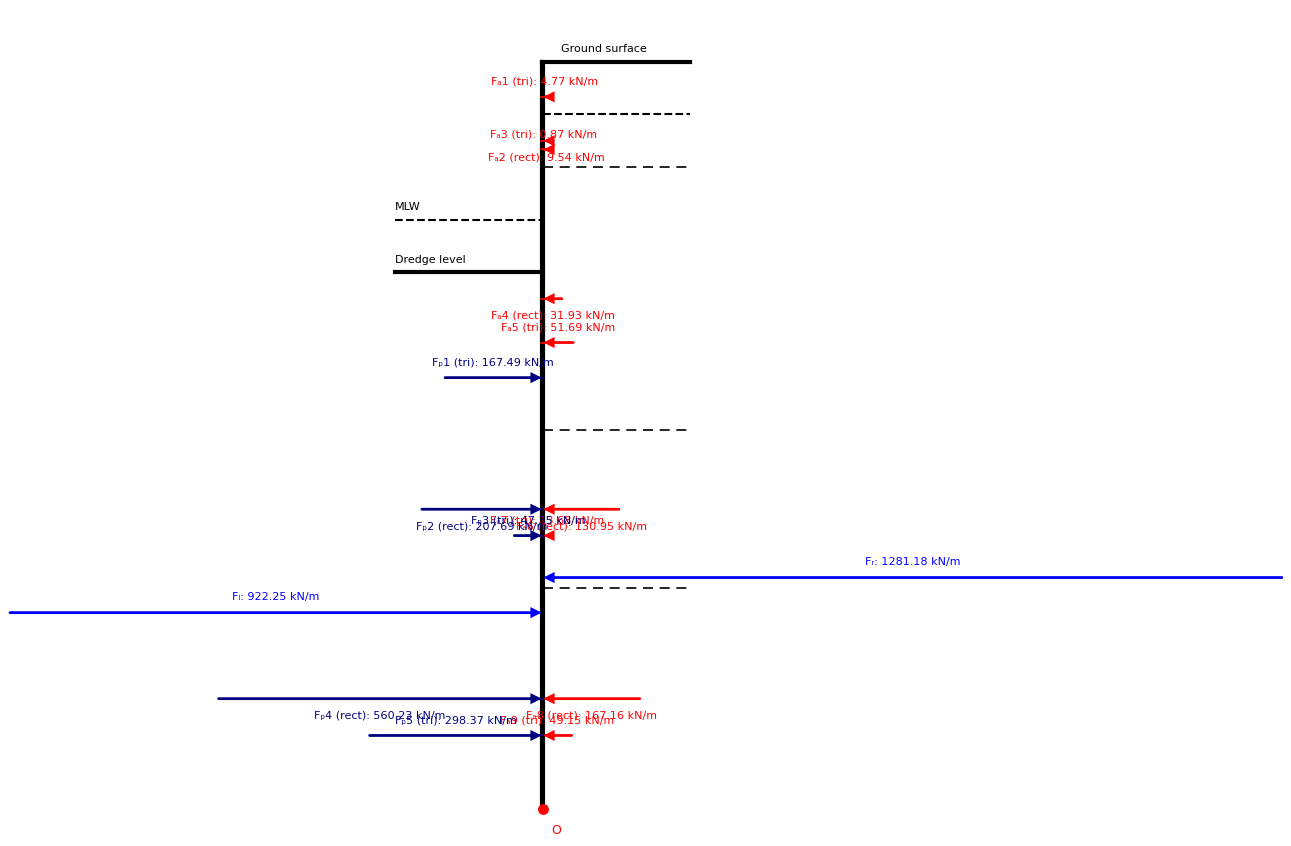
\includegraphics[width=0.80\linewidth]{figures/ch8/uls_combination_scale.png}
%     \caption{ULS combination forces for $t = 10.196$ m }
%     \label{fig:uls_moments_balance_forces}
% \end{figure}

% NAAR DE BIJLAGE

% \begin{table}[H]
%   \centering
%   \caption{Resultant forces, arms, and moments for $t = 10.196$ meters}
%   \label{tab:forces_arms_moments_new}
%   \small
%   \setlength{\tabcolsep}{6pt}
%   \renewcommand{\arraystretch}{1.15}
%   \begin{tabular}{@{}l l r r r r@{}}
%     \toprule
%     Side & Shape &
%     F [kN/m] & $z_{base}$ [m] &
%     $M_{\text{base}}$ [kN$\cdot$m/m] \\
%     \midrule
%     ACTIVE & Triangle  &   4.77  & 13.53 &   64.52 \\
%     ACTIVE & Rectangle &   9.54  & 12.70 &  121.10 \\
%     ACTIVE & Triangle  &   0.87  & 12.53 &   10.91 \\
%     ACTIVE & Rectangle &  31.93  &  9.70 &  309.57 \\
%     ACTIVE & Triangle  &  51.59  &  8.86 &  458.14 \\
%     ACTIVE & Rectangle & 130.95  &  5.70 &  745.87 \\
%     ACTIVE & Triangle  &  13.68  &  5.20 &   71.11 \\
%     ACTIVE & Rectangle & 167.16  &  2.10 &  350.69 \\
%     ACTIVE & Triangle  &  49.15  &  1.40 &   68.74 \\
%     HYDRO PASSIVE & Triangle  & 922.25 &  3.73 & -3441.82 \\
%     HYDRO ACTIVE & Triangle  & 1281.18 & 4.40 & 5635.44 \\
%     PASSIVE & Triangle  & 167.49  &  8.20 & -1372.72 \\
%     PASSIVE & Rectangle & 207.69  &  5.70 & -1182.97 \\
%     PASSIVE & Triangle  &  47.35  &  5.20 &  -246.00 \\
%     PASSIVE & Rectangle & 560.23  &  2.10 & -1175.33 \\
%     PASSIVE & Triangle  & 298.37  &  1.40 &  -417.31 \\
%     \midrule
%     $\sum M_{t}$ (should ≈ 0 for equilibrium) & & & & -0.0763 \\
%     \bottomrule
%   \end{tabular}
% \end{table}

% TABELLEN NAAR BIJLAGE

% HIER NU DE MEEST ONGUNSTIGE COMBINATIE BESPREKEN EN DE LAATSTE PLOT VAN DE MOMENTENSOM EN KRACHTENSOM OPNIEUW LATEN ZIEN NAAST ELKAAR IN EEN SUBPLOT. DAN DE DIEPTE T NOG EEN KEER BENOEMEN EN BEPALEN. OOK DE MOMENTENLIJN EN DWARSKRACHTENLIJN LATEN ZIEN.

In Table \ref{tab:uls_summary}, an overview of the ULS analysis is shown. From this overview, it can be seen that the ULS combination DA1-2 is governing, and in the following section, these moments and shear will be verified with respect to the chosen profile.

\begin{table}[H]
  \centering
  \caption{ULS results summary from design figure}
  \label{tab:uls_summary}
  \small
  \setlength{\tabcolsep}{8pt}
  \renewcommand{\arraystretch}{1.15}
  \begin{tabular}{@{}l r r r r r@{}}
    \toprule
    ULS & \multicolumn{1}{c}{Retained height [m]} & \multicolumn{1}{c}{Embedding depth [m]} & \multicolumn{1}{c}{Toe depth [m]} & \multicolumn{1}{c}{Max moment [kNm/m]} & \multicolumn{1}{c}{Max shear [kN/m]} \\
    \midrule
    DA1-1   & 4.0 & 7.58 & 11.6 & 280.5 & 220.6 \\
    DA1-2  & 4.0 & 10.17 & 14.2 & 404.4 & 266.6 \\
    \bottomrule
  \end{tabular}
\end{table}


\section{Structural Verification ULS}

In this structural verification of the cantilever sheet pile, a profile should be chosen and internally verified according to Eurocode 3. To perform the verifications, first the section of the sheet pile should be classified. After, verifications concerning the bending, shear and combined bending and shear can be performed. In these verifications the basic procedure for analyzing the profile will be that the actions do not exceed the resistance of the profile, shown in Equation \ref{limit_state}.

% HIER NOG EEN SECTION KIEZEN. ARCELORMITTAL DOCUMENT EN DE BIJKOMENDE PROPERTIES IN EEN TABEL.

\begin{equation}
    E_{d} \leq R_{d}
    \label{limit_state}
\end{equation}

\begin{itemize}
    \item $E_{d}$    design effects of actions
    \item $R_{d}$   design resistance
\end{itemize}

In this section, the cross section AZ 24-700 from ArcelorMittal is verified. As this section will be placed in the river and is assumed to have fresh water, a corrosion factor should be incorporated. This means that the properties of the cross-section after corrosion will have a loss of thickness. From Eurocode 3, the total thickness loss, for a design working life of $t_{DWL} = 50 \ years $, is calculated as follows:

\begin{equation}
    \Delta_{t} = \Delta_{tfront} +  \Delta_{tback} = 0.9 + 0.6= 1.5 \ mm 
    \label{limit_state}
\end{equation}

With a loss of thickness of $1.5 \ mm$, the properties regarding height, flange thickness, web thickness, sectional area, elastic section modulus, and plastic section modulus will be reduced. The reduced properties after erosion of this section are shown in Table \ref{tab:pu32}.

% Z PROFILES ARE STRONGER AND FOR WATER USE, DEEPER EXCAVATION

\begin{table}[H]
  \centering
  \small
  \setlength{\tabcolsep}{6pt}
  \renewcommand{\arraystretch}{1.15}
  \caption{Geometrical and mechanical properties of sheet pile section AZ 24-700}
  \label{tab:pu32}
  \begin{tabular}{@{}l l l c@{}}
    \toprule
    Property & Symbol & Units & AZ 24-700 \\
    \midrule
    Overall width                & $b$     & mm     & 700   \\
    Overall height               & $h$     & mm     & 457.5   \\
    Flange thickness             & $t_f$   & mm     & 9.7  \\
    Web thickness                & $t_w$   & mm     & 9.7  \\
    Flange breadth               & $b_f$   & mm     & 361   \\
    Slant angle                  & $\alpha$ & $^\circ$ & 55.2 \\
    Sectional area               & $A$     & cm$^2$/m & 163 \\
    Elastic section modulus      & $W_{el}$ & cm$^3$/m & 2435 \\
    Plastic section modulus      & $W_{pl}$ & cm$^3$/m & 2810 \\
    Moment of inertia            & $I$     & cm$^4$/m & 55890 \\
    Mass                         & ---     & kg/m$^2$ & 128 \\
    Class    & ---     & ---     & 3 \\
    \bottomrule
  \end{tabular}
\end{table}

% VERANDEREN NAAR AZ 24-700

\subsubsection{Section classification}

The classification of the steel profile tells whether the profile is behaving elastic or plastic. This is of importance when further analyzing the stability of the cantilever sheet pill with the bending and shear checks. The cross-section is classified by the flange slenderness ratio of the section. In Table \ref{tab:section_classification}, the classes and the ratios for Z and U profiles is shown. Formula \ref{eq:epsilon} is related to the coefficient that depends on the steel grade. 

\begin{equation}
    \epsilon = \sqrt{\frac{235}{f_{y}}}
    \label{eq:epsilon}
\end{equation}

\begin{itemize}
    \item $f_{y}$   yield strength [$N/mm^{2}$]
\end{itemize}

\begin{table}[H]
  \centering
  \small
  \setlength{\tabcolsep}{8pt}
  \renewcommand{\arraystretch}{1.15}
  \caption{Section classification}
  \label{tab:section_classification}
  \begin{tabular}{@{}l l c c@{}}
    \toprule
    \multicolumn{1}{l}{Class} &
    \multicolumn{1}{l}{Rotation check} &
    \multicolumn{2}{c}{Ratio of $b/t_f$ is less or equal than\ldots} \\
    \cmidrule(lr){3-4}
    & & Z-profile & U-profile \\
    \midrule
    \textit{1} & Required     & $45\,\varepsilon$ & $37\,\varepsilon$ \\
    \textit{2} & Not required & ---               & ---               \\
    \textit{3} & Not required & $66\,\varepsilon$ & $49\,\varepsilon$ \\
    \bottomrule
  \end{tabular}
\end{table}

For the cross-section verification, the profile AZ 24-700 with the cross-section properties from Table \ref{tab:pu32} in grade S355 GP is classified as Class 3, regarding Equation \ref{eq:class}.

\begin{equation}
    \frac{b}{t_{f}} = \frac{361}{9.7} = 37.2 \leq 66 \epsilon 
    \label{eq:class}
\end{equation}

\subsubsection{Bending}

For the verification of bending, it is important that the design bending moment, $M_{Ed}$, is smaller than the bending resistance, $M_{Rd}$, of the profile. The maximum bending moment, $M_{Ed}$, acting at the point of zero shear is $404.4 \ kNm/m$, shown in Figure XX. Within Class 3, Equation \ref{eq:bending_plastic} is used to calculate the bending resistance.

\begin{equation}
    M_{Ed} \leq M_{c,Rd}
\end{equation}

\begin{equation}
    M_{c,Rd} = \frac{\beta_{B} \cdot W_{el} \cdot f_{y}}{\gamma_{M0}}
    \label{eq:bending_plastic}
\end{equation}

\begin{itemize}
  \item $\beta_B$ is a factor that accounts for possible lack of shear force transmission in the interlocks between adjacent piles (for U-piles only);
  \item $W_{el}$ is the cross-section’s elastic section modulus;
  \item $f_y$ is the yield strength of steel;
  \item $\gamma_{M0}$ is a partial factor.
\end{itemize}

Following the equation above, the bending moment resistance of the cross-section is calculated and verified with the following equations:

\begin{equation}
    M_{c,Rd} = \frac{1.00 \cdot 2430 \cdot 355}{1.0} = 862.7 \ kNm/m
\end{equation}

\begin{equation}
    \frac{M_{Ed}}{M_{Rd}} = \frac{404.4}{862.7} = 0.47
\end{equation}

% \begin{figure}[H]
%     \centering
%     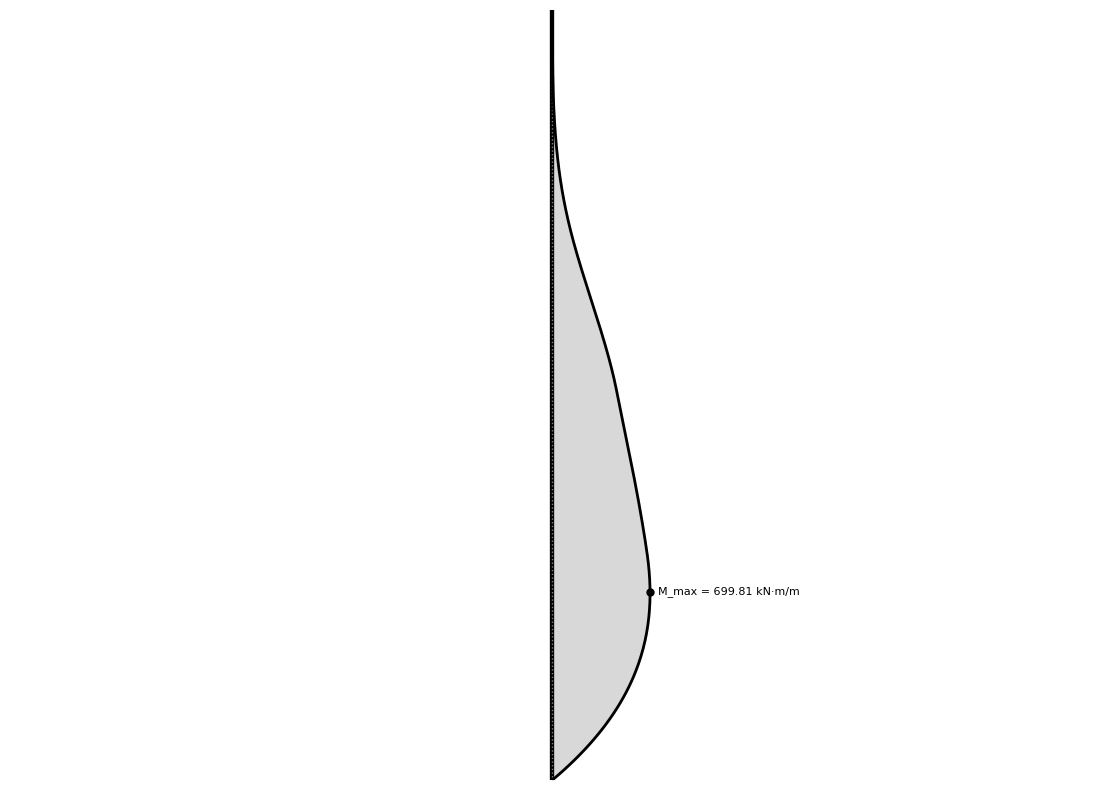
\includegraphics[width=0.90\linewidth]{figures/ch8/bending_moment.png}
%     \caption{Bending moment distribution $t = 10.196$ m}
%     \label{fig:uls_moments_line}
% \end{figure}

% FIGUUR NAAR BIJLAGE

\subsubsection{Shear}

For the verification of shear, it is important that the design shear force, $V_{Ed}$ is smaller than the plastic shear resistance, $V_{pl,Rd}$, of the profile. The maximum shear force, $V_{Ed}$, is $266.6 \ kN/m$, shown in Figure XX. Equation \ref{eq:shear_verification} is used to calculate the shear force resistance.

\begin{equation}
    V_{Ed} \leq V_{pl,Rd}
    \label{eq:shear_plastic}
\end{equation}

\begin{equation}
    V_{pl,Rd} = \frac{A_v \cdot f_{y}}{\sqrt{3} \cdot \gamma_{M0}}
    \label{eq:shear_verification}
\end{equation}

\begin{itemize}
    \item $A_{v}$ is the projected shear area of each web ($A_{v} = t_w \cdot (h-t_f)$)
    \item $t_w$ is the web’s thickness
    \item $t_f$ the flange thickness
    \item $h$ the overall height of the cross-section
\end{itemize}

Following the equation above, the shear force resistance of the cross-section is calculated and verified with the following equations:

\begin{equation}
    A_v = 9.7 \cdot (457.5 - 9.7) = 4343.7 \ mm^2
\end{equation}

\begin{equation}
    V_{pl,Rd} = \frac{4343.7 \cdot 355}{\sqrt{3} \cdot 1.0 \cdot 10^3} = 890.4 \ kN 
\end{equation}

\begin{equation}
    V'_{pl,Rd} = \frac{890.4}{0.7} = 1272 \ kN/m 
\end{equation}

\begin{equation}
    \frac{V_{Ed}}{V_{pl,Rd}} = \frac{266.6}{1272} = 0.21 
\end{equation}

% \begin{figure}[H]
%     \centering
%     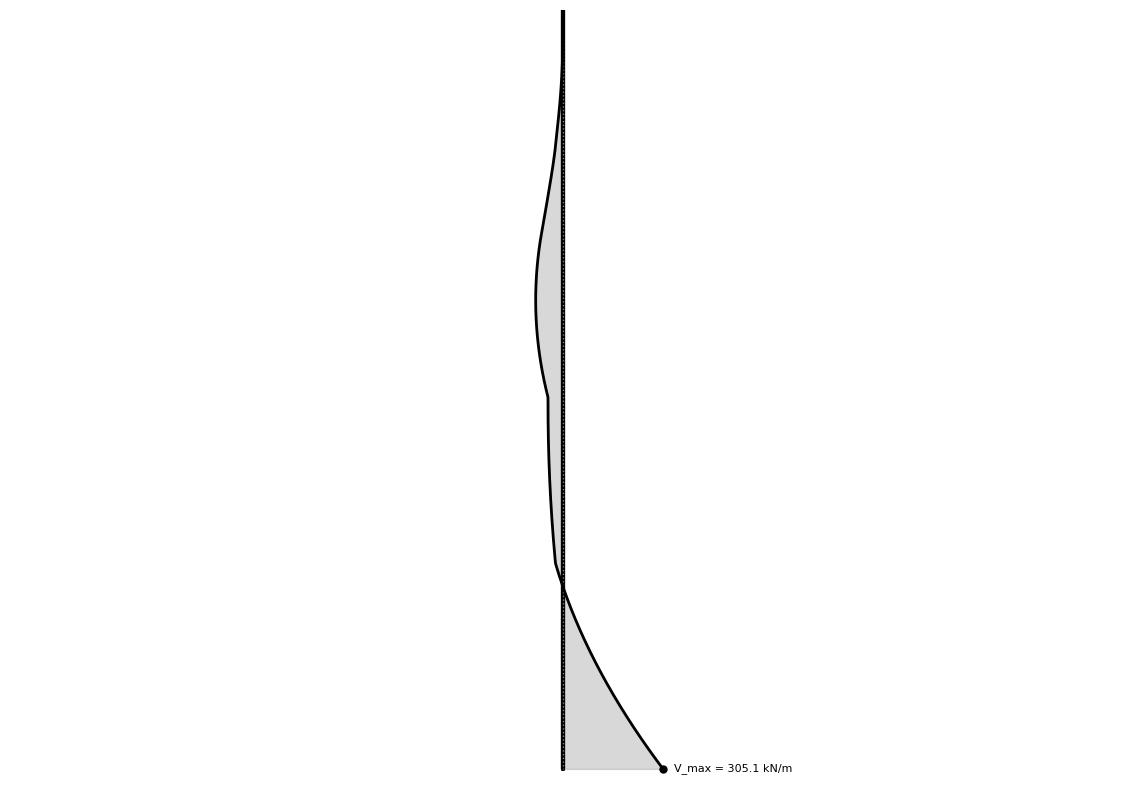
\includegraphics[width=0.90\linewidth]{figures/ch8/shear_force.png}
%     \caption{Shear force distribution $t = 10.196$ m}
%     \label{fig:uls_moments_balance}
% \end{figure}

% FIGUUR NAAR BIJLAGE

\subsubsection{Combined bending and shear}

For the verification of the combinations of bending and shear, Equation \ref{eq:combi_shear_bending} should be satisfied. However, when the cross-section is classified as plastic, the effects of shear on plastic bending resistance can be neglected if Equation \ref{eq:combi_2_shear_bending} is satisfied. 

\begin{equation}
    M_{Ed} \leq M_{V,Rd} \ , \ M_{V,Rd} \leq M_{c,Rd}
    \label{eq:combi_shear_bending}
\end{equation}

\begin{equation}
    V_{Ed} \leq \frac{V_{pl,Rd}}{2}
    \label{eq:combi_2_shear_bending}
\end{equation}

\begin{itemize}
  \item $V_{Ed}$ is the design shear force
  \item $V_{pl,Rd}$ is the design plastic shear resistance
\end{itemize}

From the following equation is may be concluded that no explicit check is needed for combined bending and moment. 

\begin{equation}
    V_{Ed} \leq \frac{1272}{2} = 636.0 \ kN/m 
\end{equation}

\subsubsection{Shear buckling}

The shear buckling resistance of the cross-section must be verified if Equation \ref{eq:shear_buckling} is valid. However, this is not satisfied, as can be seen in Equation \ref{eq:no_shear_buckling}.

\begin{equation}
    \frac{c}{t_{w}} \geq 72 \cdot \epsilon
    \label{eq:shear_buckling}
\end{equation}

\begin{equation}
    c = \frac{h - t_{f}}{sin(\alpha)} = \frac{457.5 - 9.7}{sin(55.2)} = 546.7 
\end{equation}

\begin{equation}
    \frac{546.7}{9.7} = 56.4 \ngeq 72 \cdot \epsilon 
    \label{eq:no_shear_buckling}
\end{equation}

\subsubsection{Local effects of water pressure}

As in the geometry of the cross-section, there is a difference in water levels on both sides of the sheet pile, the bending moments should be reduced by transverse local plate bending. Therefore, the cross-sectional yield strength should be reduced with Equation \ref{eq:reduction_factor}. However, when the difference in the water levels across the wall, for Z sections, is less than $5.0 \ m$. From Equation XX it can be seen that the difference in water levels is less than $5.0 \ m$, showing that the local effects of water pressure on overall bending may be neglected. 

\begin{equation}
    f_{y;red} = \rho_{p} \cdot f_{y}
    \label{eq:reduction_factor}
\end{equation}

\begin{itemize}
    \item $\rho_{p}$ is a reduction factor that depends on the slenderness ratio. 
\end{itemize}

\begin{equation}
    \Delta h_w = 1.03 - 0.14 = 0.89 \ m
    \label{eq:reduction_factor}
\end{equation}

\subsubsection{Deflection}

\begin{equation}
    u_{max} \leq u_{grems}
\end{equation}

\section{Verification D-Sheet Software}

\section{Final design}

\newpage

\section{Nature-based Solutions}

When it comes to Nature-based solutions, the question arises what this definition means. A general definition of Nature based Solutions is;

\textit{“Nature-based Solutions are actions to protect, conserve, restore, sustainably
use and manage natural or modified terrestrial, freshwater, coastal and marine
ecosystems, which address social, economic and environmental challenges
effectively and adaptively, while simultaneously providing human well-being,
ecosystem services, resilience and biodiversity benefits” \autocite{eiselinVerenigdeNatiesStemmen2022}}

Although the name may give a thought that it only concerns natural and biodiversity increasing ideas this is actually not the case. For example the impact of NBS on the local economies and communities is of an equal importance. When it comes to weighing the different NBS against each other this report will make use of the seven goals of the IUCN which must be achieved as good as possible. The seven goals are presented below;

\begin{figure}[H]
    \centering
    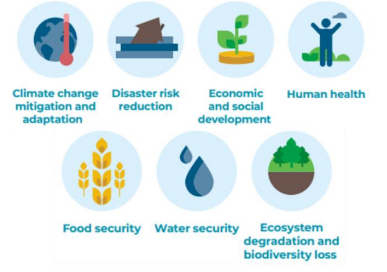
\includegraphics[width=0.50\linewidth]{figures/ThesevenNBSgoals.png}
    \caption{Seven goals for achieving a good NBS \autocite{.....}}
    \label{fig:7g}
\end{figure}

\subsection{Resistance against NBS}

Although NBS are widely known in the scientific world, most people have never heard of these solutions. So, when implementing a solution which can't be described as a classical solution, there is a big change of getting resistance from multiple stakeholders. Especially local communities are skeptical because the solution is less concrete than a classical solution would be. The business case of a NBS must of course also be solid. Without funding of the project, there will never be a change to realize it. That's why it's from great importance to have a solution which is both reachable and explainable to the stakeholders. 

\subsection{Implementing NBS in this project}

As stressed out before, there is a problem with riverbank erosion due to processes of the river. Besides that there are also several problems due to dry sand mining. To mitigate or even solve these problems, it is the group's intend to use a nature based solution. Therefore there are presented multiple possible solutions to create a long-lasting, sustainable riverbank which is made cost effective. These solutions are all graded from one to ten for the seven goals described in Figure \ref{fig:7g}. 


\section{Bed and bank protection measures}
The Paraná Delta, the end of the Paraná-Paraguay river wetland system, begins in the city of Diamante in Entre Ríos province. It stretches for 300 kilometres and covers some 2.3 million hectares. Dotted with islands, these wetlands are a source of ecosystem services such as flood and drought buffering, water purification, erosion control and coastal protection, climate regulation, as well as the provision of shelter, feeding and breeding sites for various wildlife species. It also provides resources including fish, foraging, timber, medicine, and materials for construction and clothing \autocite{hibaParanaRiverEcological2024}.

In recent years, wetlands have become increasingly important for another key reason: their role as allies against climate change. They improve the resilience of communities to its impacts, serve as natural barriers against floods and droughts, and also function as carbon sinks. Despite playing these important roles, these ecosystems remain under great threat from human action – it is estimated that globally, 85 percent of the wetlands that existed three centuries ago have been destroyed or drastically transformed \autocite{hibaParanaRiverEcological2024}.

\section{Nature-based Solutions for dry sand mining}
%Meer overheidsingrijpen nodig? Zie interview burgemeester: The judiciary forced the government to get involved: do controls, plan and regulate. Now there’s a limit to extract, approx. 2 – 3 m. Before, there wasn’t. En sed de arena report, overheid niet proactief genoeg

%https://www.unep.org/resources/report/sand-and-sustainability-10-strategic-recommendations-avert-crisis
%https://aapepyg.com/2022/11/23/fracking_entre_rios/#_edn4

%While significant strides are taken to implement nature-based solutions (NbS) against climate change challenges, it is important to note that NbS requires large volume of sand. Additionally, NbS may take time to have the desired effect. Thus in some cases, grey structures (i.e., concrete) may be necessary in the mean time to address challenges in the short- to medium-term. In the context of extreme heat and its impacts on cities, NbS will also be instrumental to promote building designs and materials that require neither concrete infrastructure nor sand (UNEP 2021b). Climate change induced pressures, such as temperature stress and precipitation, will also speed up the degradation of existing infrastructure and the need for upgrading or replacement https://www.unep.org/resources/report/sand-and-sustainability-10-strategic-recommendations-avert-crisis

%Op basis van uitgebreid, door deskundigen beoordeeld bewijsmateriaal concludeerde het Compendium van wetenschappelijke, medische en media-bevindingen die de risico's en schade van fracking aantonen, dat het niet mogelijk is om de techniek van de winning van onconventionele koolwaterstoffen 17Sed de Arena 2023 I Valeria Foglia en de daarmee samenhangende winningsactiviteiten niet mogelijk is zonder dat dit een bedreiging vormt voor de menselijke gezondheid, de lucht, het water, de economische vitaliteit op lange termijn, de biodiversiteit en de seismische en klimatologische stabiliteit. SED DE ARENA

This section seeks to propose and evaluate Nature-Based Solutions (NBS) that can effectively address the environmental and socio-economic consequences of dry sand mining. The analysis focuses on developing strategies that harness natural processes to restore degraded ecosystems, enhance landscape resilience, and promote sustainable resource management. In order to provide a comprehensive understanding, the potential advantages and limitations of each proposed NBS will be critically examined. Furthermore, this section will delineate the intended implementation framework, outlining the methodological approach and practical steps required to translate these solutions into effective, context-specific interventions.

\subsection{Floodplains}

Floodplains are low-lying areas around rivers that naturally flood during periods of high water discharge. When managed and restored appropriately, these zones play a crucial role in maintaining riverine ecosystem functions and mitigating the adverse impacts of human activities such as sand mining and land degradation.

In the context of dry sand mining, floodplains could be a Nature-Based Solution to counteract the degradation of terrestrial and hydrological systems resulting from excessive sand extraction. Dry sand mining frequently occurs in former floodplain areas or adjacent uplands, where the removal of surface materials disrupts soil structure, alters drainage patterns, and reduces the area’s natural capacity to retain water. Restoring and reactivating floodplains in such landscapes helps to re-establish the natural hydrological connectivity between surface and subsurface systems. This process promotes groundwater recharge, initiate soil sedimentation and mitigates erosion caused by wind and surface runoff. Moreover, re-vegetated floodplains provide new habitats for native species, contributing to the overall ecological recovery of mined areas. As such, floodplain restoration in dry sand mining zones supports landscape resilience, reduces the long-term environmental footprint of extraction activities, and facilitates a more sustainable post-mining land use.

Restored floodplains offer significant opportunities for local community engagement, livelihood diversification, and socio-economic development. Once stabilized and revegetated, these areas can be utilized for sustainable land uses such as flood-resilient agriculture, agroforestry, and controlled grazing, which maintain ecological functions while providing income for local populations. Additionally, floodplains can serve as sites for eco-tourism, recreation, and environmental education, fostering a stronger connection between communities and their natural surroundings. The enhancement of biodiversity and landscape aesthetics further increases the cultural and recreational value of these areas. Moreover, the restored floodplain’s role in improving water retention and soil fertility can directly support local food and water security, especially in regions affected by the environmental degradation of dry sand mining. Through community-based stewardship, floodplain restoration can therefore become a catalyst for sustainable rural development and long-term environmental resilience.

\subsection{Metal-tolerant plants}
As mentioned in section \ref{sect:dryminingeffects}, iron concentrations in the ground water have increased by 2200\% since sand mining operations have started. Meanwhile, manganese concentrations are above the recommended concentration limits and polyacrylamide poses a danger to the users' health. Clearly, there is a need for limiting the amount of metal elements and polluters that infiltrate the groundwater.

The use of metal-tolerant plants, such as phytostabilizers and hyperaccumulators, represents an effective Nature-based Solution for mitigating contamination and surface runoff in areas affected by dry sand mining. These plant species have the capacity to absorb, immobilize, or stabilize pollutants, including heavy metals and chemical residues from washing processes, within their roots or above-ground tissues. By establishing vegetation on disturbed or contaminated soils, this method reduces the mobility of harmful substances, prevents their leaching into nearby water bodies and the aquifer, and enhances overall soil stability.

In addition to pollutant control, these plants help reduce surface runoff by increasing soil infiltration capacity and root cohesion, thereby minimizing erosion and the spread of sediments. Over time, the vegetative cover contributes to ecosystem recovery, transforming degraded mining landscapes into self-sustaining, biologically active systems.
Within the Paraná Delta, several naturally occurring plant species exhibit tolerance to moderate metal contamination, conditions which can be associated with post-mining sites. Examples include:

\begin{itemize}
    \item Phragmites australis (reed): known for high tolerance to heavy metals and ability to stabilize sediments \autocite{popaHeavyMetalsAccumulation2023}.
    \item Typha domingensis (southern cattail): native to wetlands in a delta; capable of uptaking and accumulating metals \autocite{solimanTyphaDomingensisPers2024}.
    \item Schoenoplectus californicus (California bulrush): efficient in reducing nutrient and contaminant loads in water.
    \item Spartina densiflora (cordgrass): salt- and metal-tolerant grass found along deltas and coastal zones.
\end{itemize}

These species are native or naturalized in the Paraná Delta region and can therefore be used without compromising local biodiversity or ecological integrity \autocite{m.eidPhytoremediationHeavyMetals2020}. 

\subsection{Vegetated buffer zones}
Vegetated buffer zones are strips of land planted with dense vegetation, such as grasses, shrubs, and trees, established between areas of active land use (dry mining sites) and surrounding environments such as settlements, agricultural fields and nature. In the context of dry sand mining, these buffers function as a natural barrier that mitigates the spread of dust, noise, and pollutants generated by extraction activities.

From an ecological perspective, vegetated buffer zones play a vital role in stabilizing soil, reducing wind speed, and capturing airborne particles, thereby improving local air quality and minimizing off-site impacts. The root systems of the plants anchor the sandy substrate, preventing erosion and surface runoff, while the vegetation canopy traps dust and enhances microclimatic conditions by increasing humidity and reducing temperature fluctuations.

In addition to their environmental benefits, buffer zones contribute to biodiversity enhancement by creating transitional habitats that support a variety of species and small fauna. They also serve as visual and acoustic screens, reducing noise and improving the aesthetic quality of the landscape. When designed with native and drought-tolerant species, vegetated buffers require minimal maintenance and can thrive in the disturbed conditions typical of mining landscapes.

Moreover, the establishment of buffer zones can provide socio-economic advantages for local communities through community-based planting initiatives. Overall, vegetated buffer zones represent a cost-effective and multifunctional Nature-Based Solution that simultaneously addresses environmental degradation, air quality concerns, and landscape restoration in areas affected by dry sand mining.

\subsection{Implementation in Ibicuy area}
The area shown in Figure \ref{fig:PAI} includes the Cristamine S.A. sand mine (located an the right down corner) and another sand extraction site located just next to the primary school (Escuela Primaria). These mining activities have a strong influence on the surrounding landscape and local air quality. By changing the orange surrounded area into a floodplain and the blue lines into vegetated buffer zones these influences could be mitigated. 

The restoration approach by involving floodplains could be used between the area of primary school and the Cristamine mine, with the road as its boundary, as a floodplain restoration zone (orange area). This solution would be particularly valuable after mining operations have ended, allowing the area to naturally recover, increase biodiversity, and provide flood protection and water storage capacity.

In the shorter term, the vegetated buffer solution could effectively reduce dust emissions and protect the local community. Establishing dense vegetation, around the primary school would help minimize dust dispersion into the school grounds, improving air quality for the children and teachers.
Similarly, implementing vegetated buffers along the main road would limit dust movement caused by sand transportation, improving air quality, visibility and nuisance for nearby residents and road users.

From an economic feasibility perspective, these solutions are relatively cost-effective compared to large-scale engineering interventions. Vegetated buffers require moderate initial investment in planting and maintenance but offer long-term benefits in ecosystem services, reduced health costs, and improved landscape aesthetics. Floodplain restoration needs a bigger investment amount. This could be funded through mine closure obligations or environmental offsets, making it a sustainable and financially viable option for the area.


\begin{figure}[H]
    \centering
    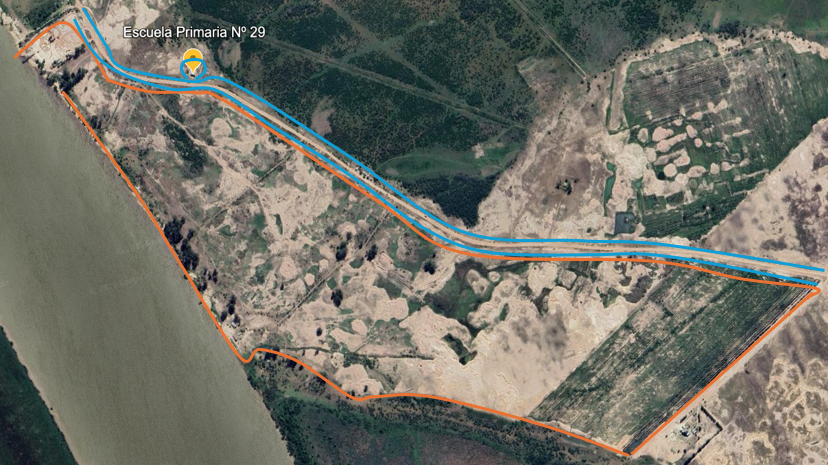
\includegraphics[width=0.75\linewidth]{figures//ch8/omgevingschooltje2.png}
    \caption{Implementation area of possible NBS}
    \label{fig:PAI}
\end{figure}

\section{Nature-based Solutions for bank erosion}
In this section, the NBS for the bank erosion, the biggest negative consequence and concern due to the river sand mining will be presented. 

\subsection{Natural Flood Management}
Natural Flood Management (NFM) is a NBS that consists of using natural materials to slow the flow of water through the land and reduce the chance of flash flooding, as well as increasing water storage throughout the landscape \autocite{therivertrust5EasyWays}. Using NFM upstream means that water takes a lot longer to reach lowlands and downstream areas. 
A number of techniques are used in NFM, such as:

\subsubsection{Natural leaky dams}
Leaky dams – placing a series of logs across a watercourse mimics the effect of naturally fallen trees. Whilst it’s important not to block the water completely, slowing the flow eases pressure downstream and reduces the risk of flooding, especially after heavy rain. Given the pathway of the cargo boats found on Marine Traffic: going along the Rio Parana Guazu, leaving out the Rio Ibicuy, but also sometimes until Puerto Ibicuy. This tells us that there is no possibility to adopt this method in the Rio Parana Guazu given that these ships would harm the NBS.

\subsubsection{Mangrove}

Planting mangroves and local vegetation along the riverbanks, particularly in areas with shallower edges. Mangroves are highly effective at stabilizing shorelines due to their dense root systems which trap sediments and reduce wave energy, like those from the cargo ships. If the right trees (Rhizophora mangle known as red mangrove, Avicennia germinans called black mangrove), are planted in the right places, a mangrove creation can go a long way towards managing the flow of water through river catchments \autocite{ferreiraPropagulosMangueVermelho2024}.
Their Leaves have the ability to intercept rainwater and soak some of it up, which slows the rate at which the rain hits the ground and enters rivers. Below ground, tree roots help to bind soil together, reducing the amount of sediment which runs off into watercourse. A Figure \ref{fig:Rhizophora mangle} of a Rhizophora mangle (red mangrove) and a Figure \ref{fig:Avicennia germinans} of Avicennia germinans (black mangrove) are shown below:

\begin{figure}[H]
    \centering
    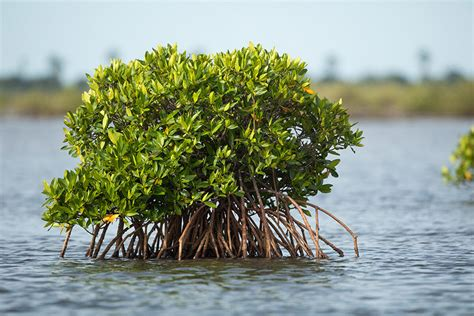
\includegraphics[width=0.75\linewidth]{figures/ch8/mangrove1.jpeg}
    \caption{Implementation area of possible NBS}
    \label{fig:Rhizophora mangle}
\end{figure}

\begin{figure}[H]
    \centering
    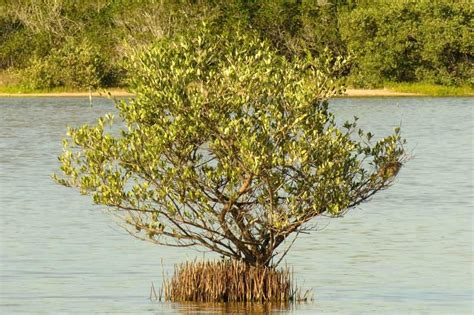
\includegraphics[width=0.75\linewidth]{figures/ch8/mangrove2.jpeg}
    \caption{Implementation area of possible NBS}
    \label{fig:Avicennia germinans}
\end{figure}

Putting the idea to the test, the locations where these mangroves would be the most useful would of course be where the bank erosion is the worst. In this case that would be the outside of the river turns of the region of interest. That would include locations like the land of stakeholders such as the owner of the Camping La Blanqueada, Camping El Trebol, Camping Ipona Guazu, or Oasis Guazu. 

\subsubsection{Deposited Rock Debris as a NBS}
In Camping Oasis Guazu, mitigations strategies have already been tested. The owner chose to put rocks on the side of the bank to decrease the erosion process as seen in Figure \ref{fig:local solution Camping Oasis Guazu}.

\begin{figure}[H]
    \centering
    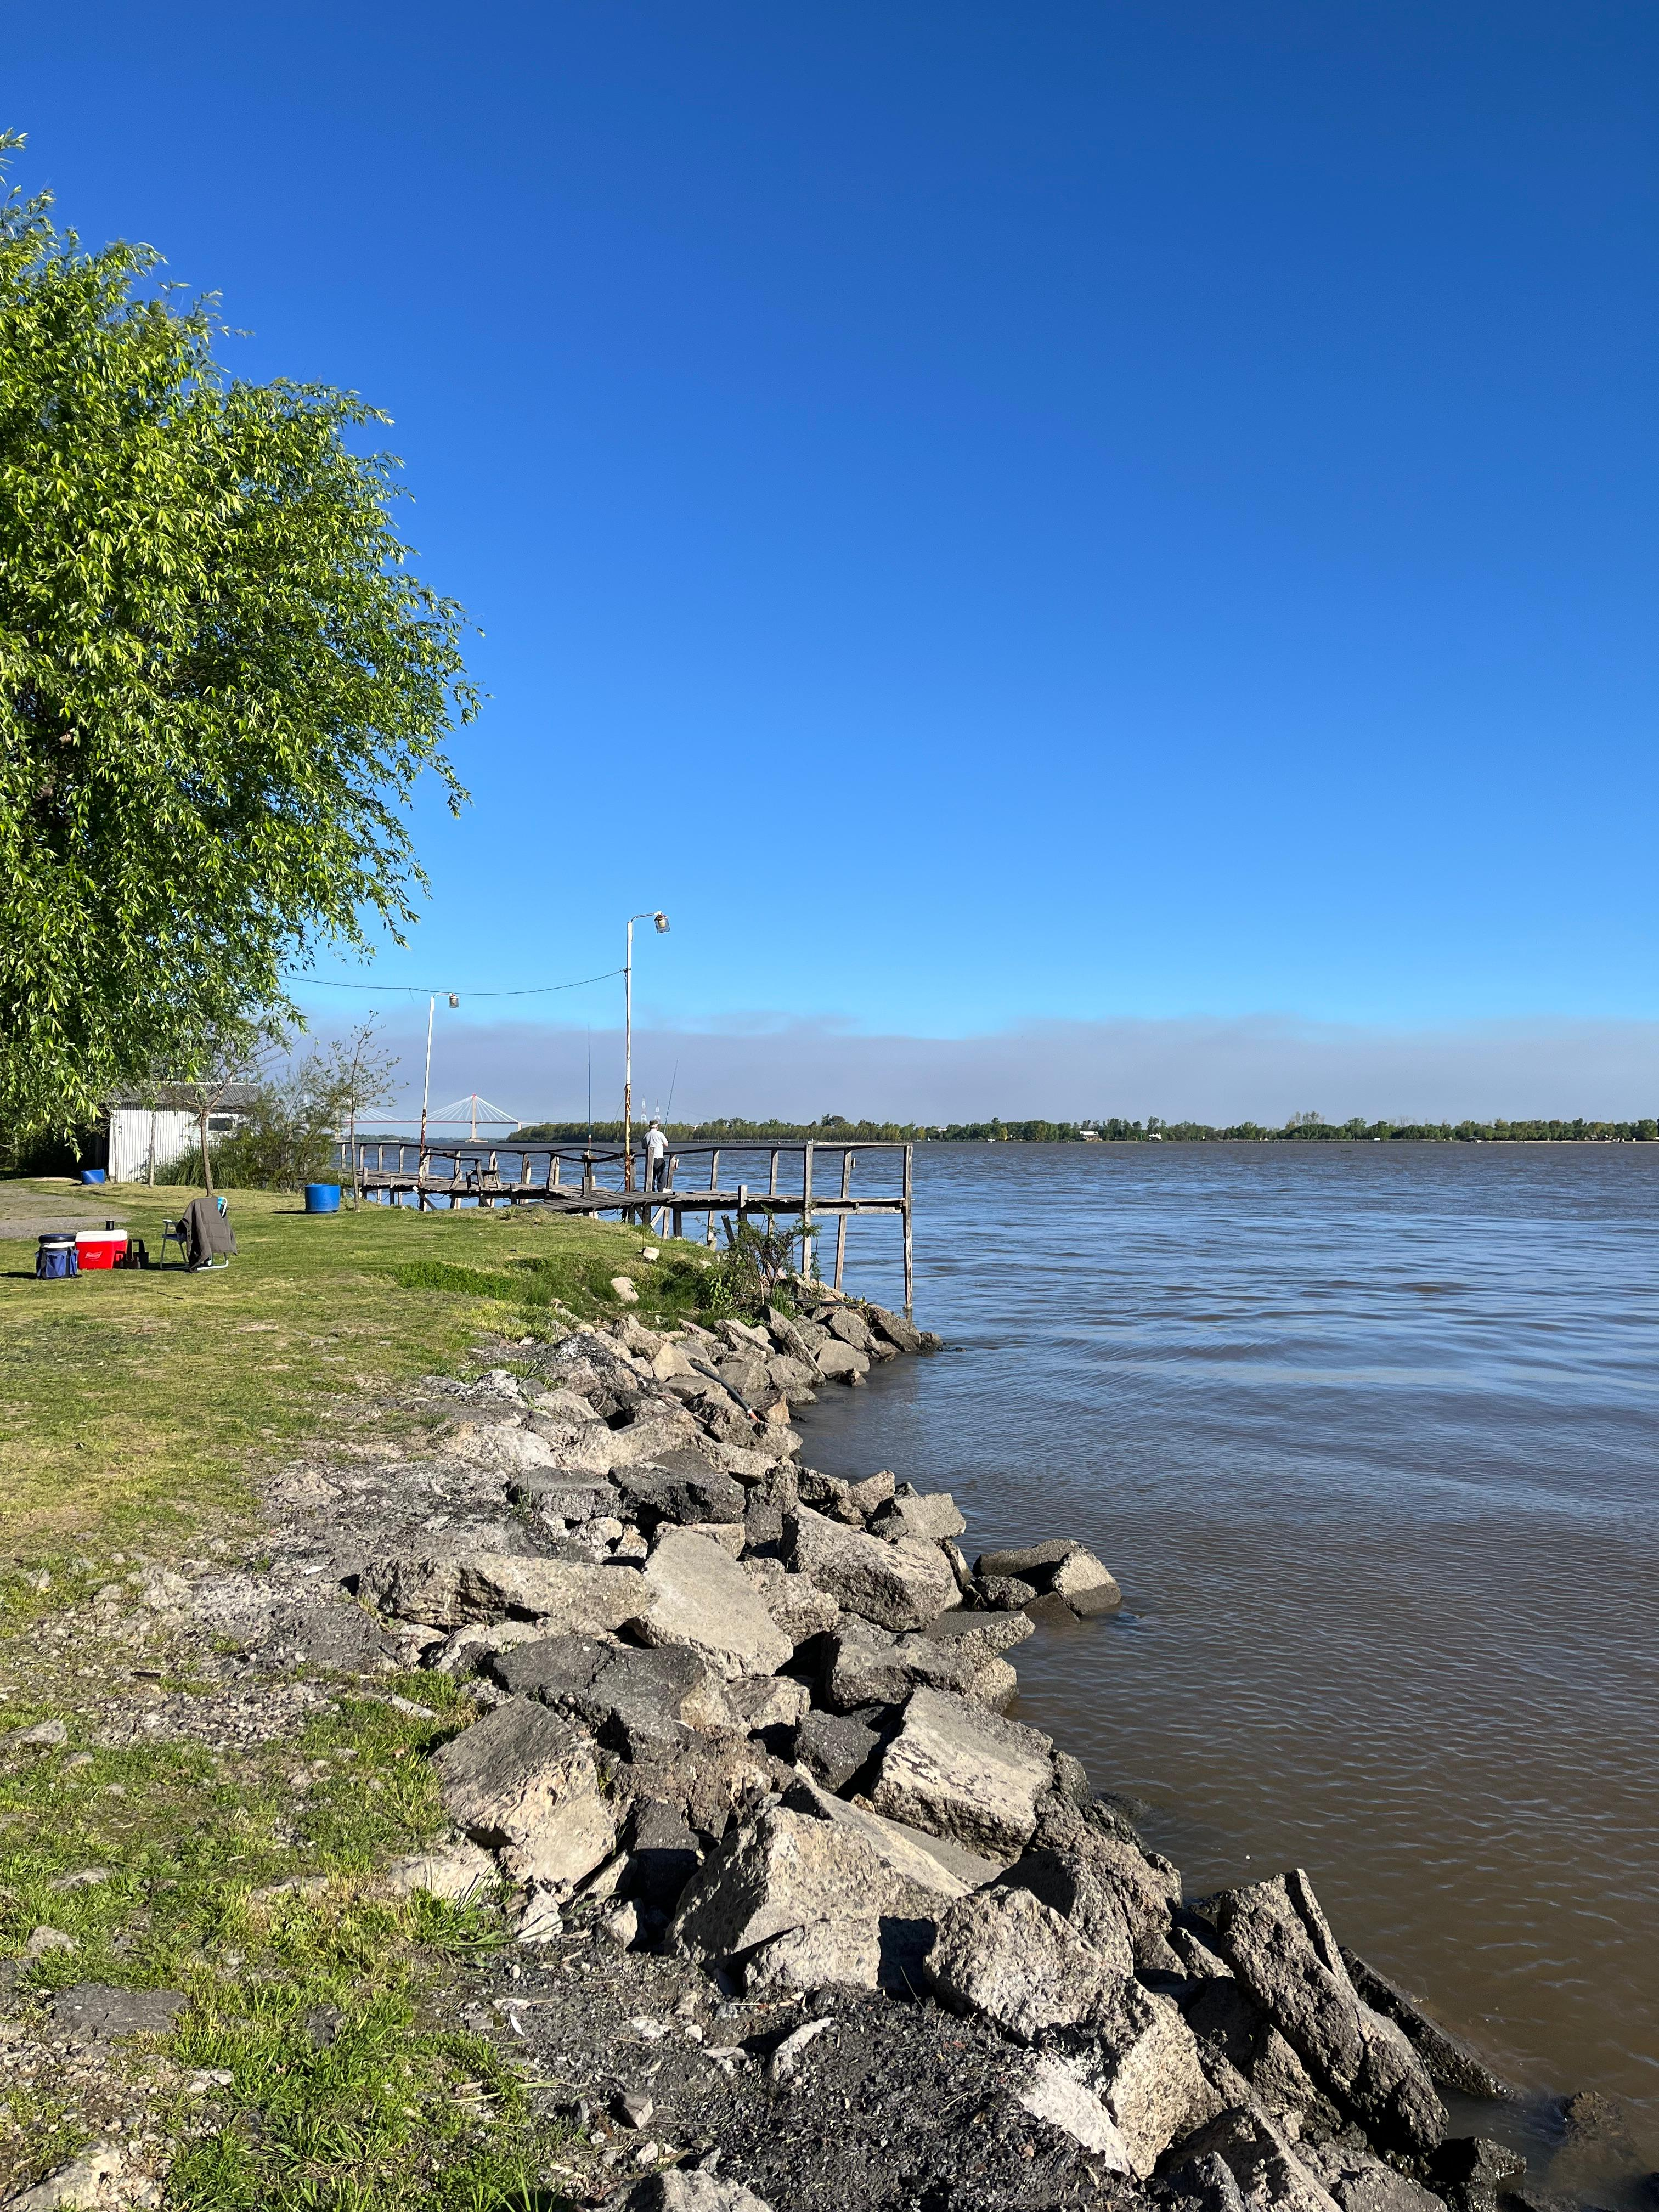
\includegraphics[width=0.75\linewidth]{figures/appendixE/rocks.jpg}
    \caption{Local solution Camping Oasis Guazu}
    \label{fig:local solution Camping Oasis Guazu}
\end{figure}

According to the owner of the land, this solution has significantly contributed to the decrease of land erosion. As this is not a true natural solution, it could not be interpreted as a NBS like this. Nevertheless, incorporating rocks as a buffer for the current, leaving other vegetation more time to take over and contribute to the stability of the banks, that would be a suitable approach to transition towards a 100\% true NBS.


\subsubsection{Wetlands}
Making space for storing water – Features such as ponds and wetlands can store a vast amount of water which would otherwise rush through catchments as surface water. As the water passes through the wetland or pond, it is naturally filtered, often leading to lower levels of harmful pollutants. What’s more, filling the pond or wetland with native plant species encourages wildlife and provides health and wellbeing benefits too.

this part needs to be studied a bit more.

\subsubsection{Integrating the NBS into a bank design}

The final goal of this section is to integrate these solutions into the landscape. This could help establish a clearer picture of what can be achieved with these solutions.

Create a map of the region, incorporating the different options with colours and a legend.